\section{Diagrammi di sequenza}
In questa sezione vengono descritte e rappresentate tramite diagrammi di sequenza \gl{UML} le principali azioni lato back-end con lo scopo di facilitare la comprensione del funzionamento del \gl{sistema}. Per quest'ultimo motivo i diagrammi di sequenza non rappresentano l'effettiva realtà ma una sua approssimazione che non rifletterà appieno l'implementazione.
\subsection{Interazioni passate con la persona interagente}
Il diagramma qui riportato rappresenta la chiamata al \gl{webhook} da parte di api.ai per la ricerca di interazioni passate con la persona interagente . L'interazione inizia con la chiamata del metodo \file{webhook} fornito dalla classe \file{ConversationWebhookService} da parte di \file{api.ai}. Il metodo si occupa di ottenere la lista degli \file{User} con il metodo \file{getUserList} fornito dalla classe \file{UsersDAO}. Una volta ottenuta la lista degli \file{Users} viene controllato se la persona interagente è un amministratore. Se lo è il \file{context} della \file{lambda function} viene settato ad \file{admin}, in modo che api.ai riconosca l'utente come un potenziale amministratore e gli chieda se vuole entrare nell'area di amministrazione. Se non è un amministratore viene richiesta la lista dei \file{Guest} attraverso il metodo \file{getGuestList} fornito dalla classe \file{GuestsDAO}. Una volta ottenuta la lista viene controllato se la persona interagente è un ospite con cui si ha già avuto una o più interazioni passate. Se ciò è avvenuto il \file{context accoglienza} viene riempito con l'azienda e i dati della persona con cui l'ospite ha avuto il maggior numero di incontri in passato, e viene chiesto di confermare se la persona indicata è quella a cui l'ospite è effettivamente interessato. Se il suo nome invece non viene trovato nella lista dei \file{Guests}, la persona interagente verrà trattata come un nuovo ospite.
\begin{figure}[h] \centering 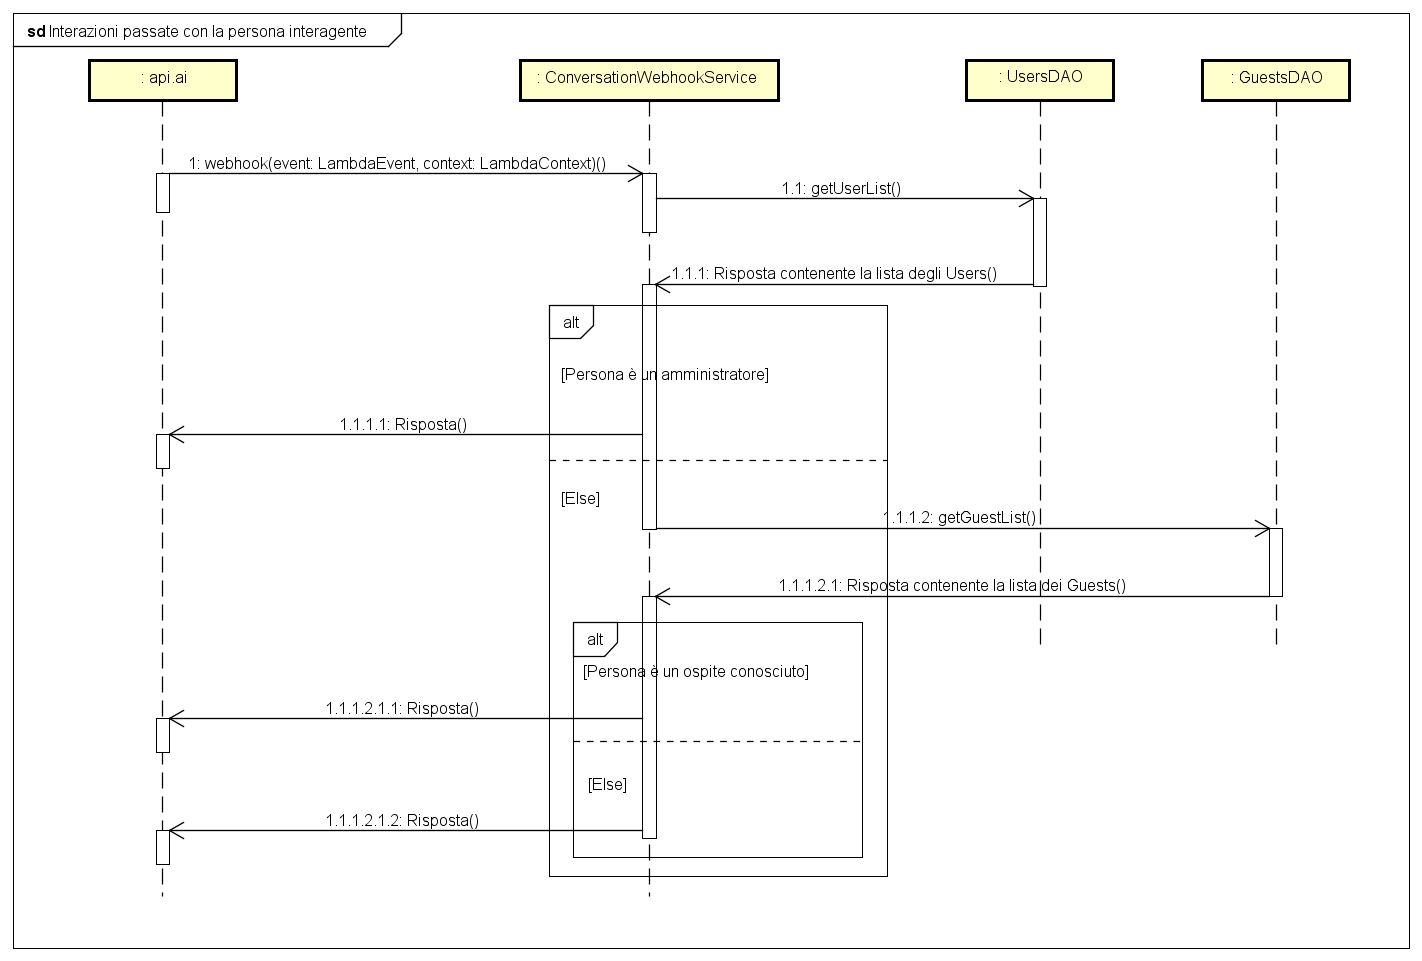
\includegraphics[width=\textwidth,height=\textheight,keepaspectratio]{images/diagrams/back-end/Ufficial_Backend/Interazionipassateconlapersonainteragente.png}
\caption{Interazioni passate con la persona interagente}
\end{figure}
\subsection{Interazione tra service e client}
Il diagramma qui riportato rappresenta l'interazione tra service e client per mezzo della chiamata al metodo \file{queryLambda} fornito dalla classe \file{VocalAPI}, il quale permette di dedurre il servizio necessario al client vocale e successivamente offrire il servizio qualora il service ne sia in grado. Per il riconoscimento dell'azione viene invocato il metodo \file{speechToText} della classe \file{STTModule}, che ritorna l'azione necessaria al client vocale a partire da un file audio. Una volta ottenuta l'azione viene controllato il valore del campo \file{action} di tale risposta. Nel caso in cui \file{action} non corrisponda ad una delle azioni supportate, ovvero action è un'azione che non richiede operazione da parte del back-end oppure \file{actionIncomplete} è impostato a true, tale risposta viene rielaborata ed inoltrata al client. Se invece l'action è supportata, il metodo si occupa di eseguire le azioni necessarie utilizzando i metodi privati della classe \file{VocalAPI}. In quest'ultimo caso viene inoltre pubblicato un messaggio su un topic di \file{SNS}, utilizzando il metodo \file{publish}, in modo che sia possibile registrare i dati relativi a tali interazioni e mandare le notifiche ai membri interessati. 
 \begin{figure}[h]
  \centering
  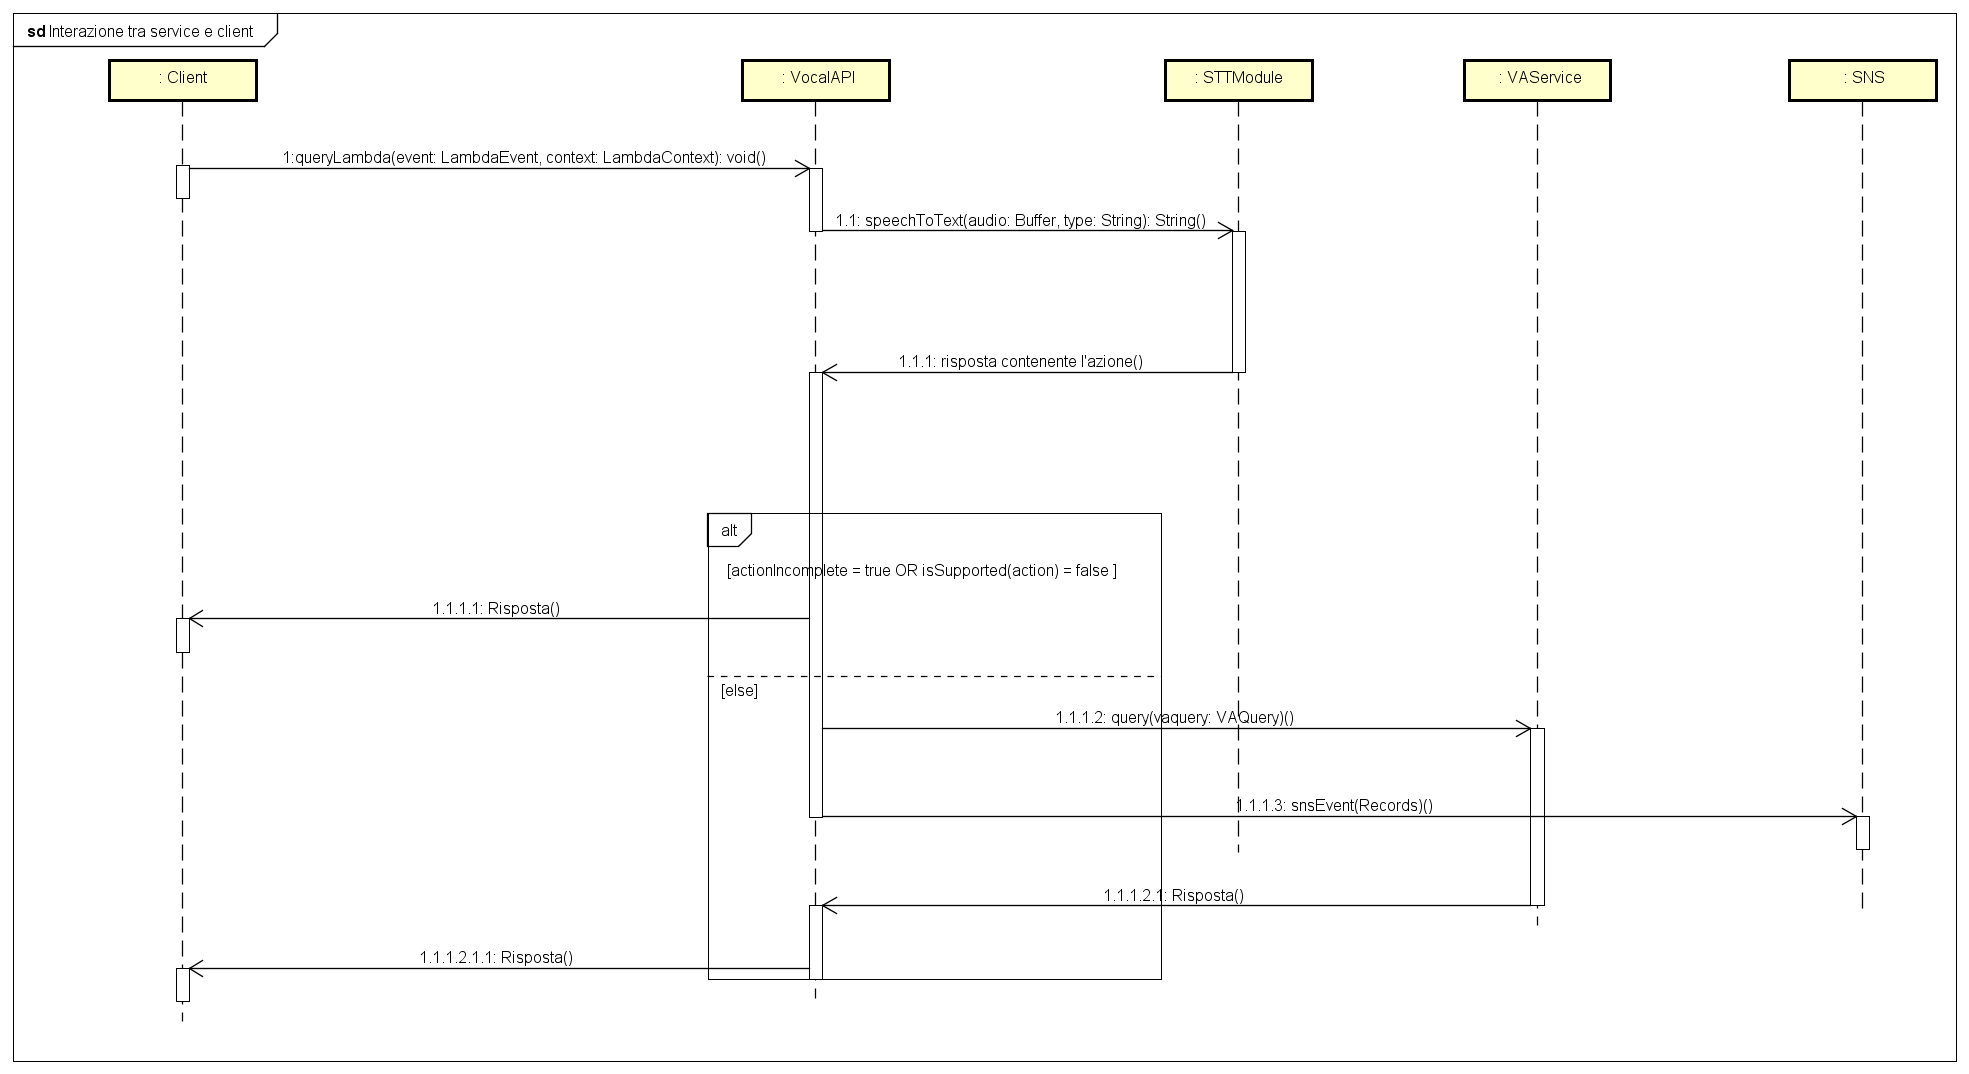
\includegraphics[width=\textwidth,height=\textheight,keepaspectratio]{images/diagrams/back-end/Ufficial_Backend/Interazionetraserviceeclient.png}
 \caption{Interazione tra service e client}
\end{figure}
\newpage
\subsection{\gl{Verifica} autenticazione}
Il diagramma qui riportato rappresenta la \gl{verifica} di un'autenticazione ad ogni interazione dell'agent di amministrazione per via del webhook fornito dalla classe \file{AdministrationWebhookService}. Tale metodo si occupa di verificare che nella richiesta sia presente un \gl{JSON} Web Token (\file{JWT}) che confermi un'autenticazione avvenuta con successo. In caso di mancata autenticazione, il campo \file{status} della risposta sarà impostato a 403. Nel caso in cui il token sia presente e valido, ovvero che la firma sia valida ed il token non sia scaduto, tale campo sarà invece impostato a 200, ed il campo \file{speech} della risposta sarà copiato da \file{fulfillment.speech} della richiesta, risultando quindi in una risposta uguale a quella definita nell'agente di api.ai.
 \begin{figure}[h] \centering 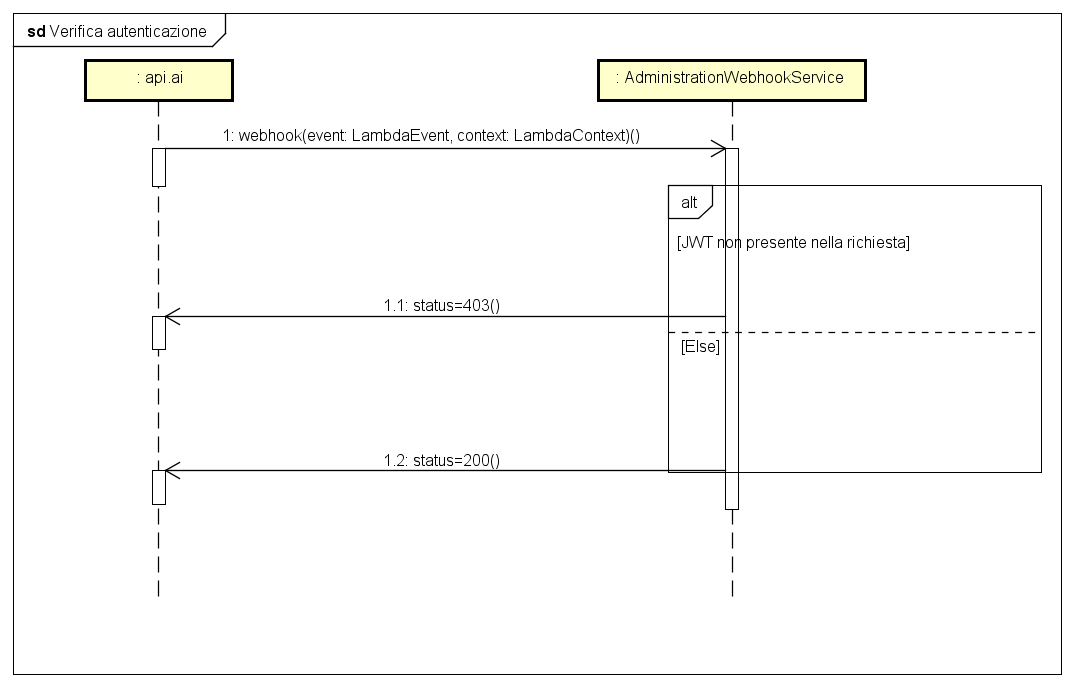
\includegraphics[width=\textwidth,height=\textheight,keepaspectratio]{images/diagrams/back-end/Ufficial_Backend/Verificaautenticazione.png} 	\caption{Verifica autenticazione}
\end{figure}
\newpage


\subsection{Back-end::Auth::UsersService::addUser}
Il diagramma qui riportato rappresenta l'implementazione della lambda function che si occupa di aggiungere un \file{User} al sistema attraverso il metodo \file{addUser}. 
 \begin{figure}[h] \centering 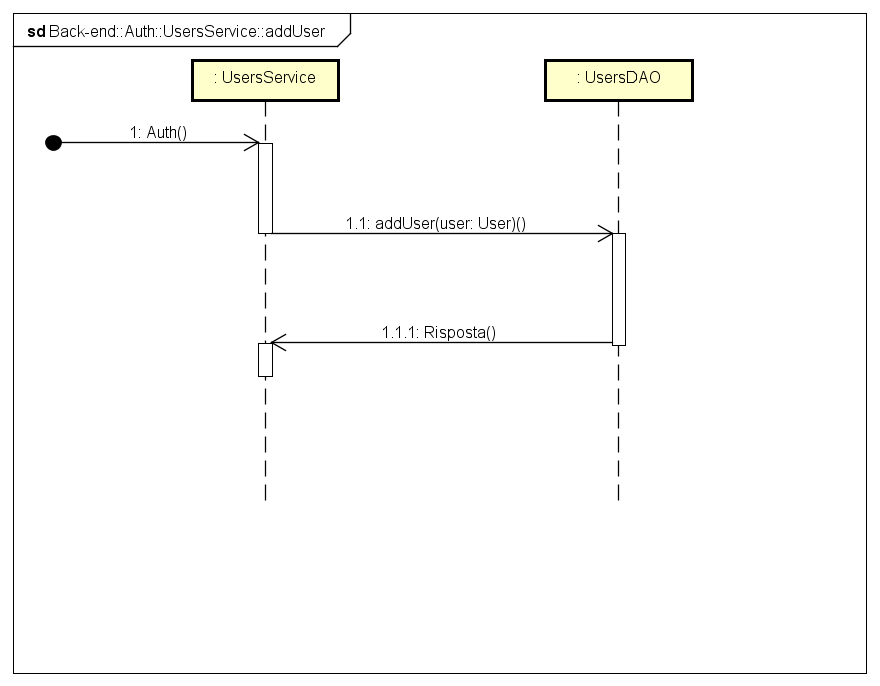
\includegraphics[width=\textwidth,height=\textheight,keepaspectratio]{images/diagrams/back-end/Ufficial_Backend/Back-endAuthUsersServiceaddUser.png} 	\caption{Back-end::Auth::UsersService::addUser}
\end{figure}

\newpage
\subsection{Back-end::Auth::UsersService::getUser} 
Il diagramma qui riportato rappresenta l'implementazione della lambda function che si occupa di ottenere un \file{User} del sistema attraverso il metodo \file{getUser}.  \begin{figure}[h] \centering 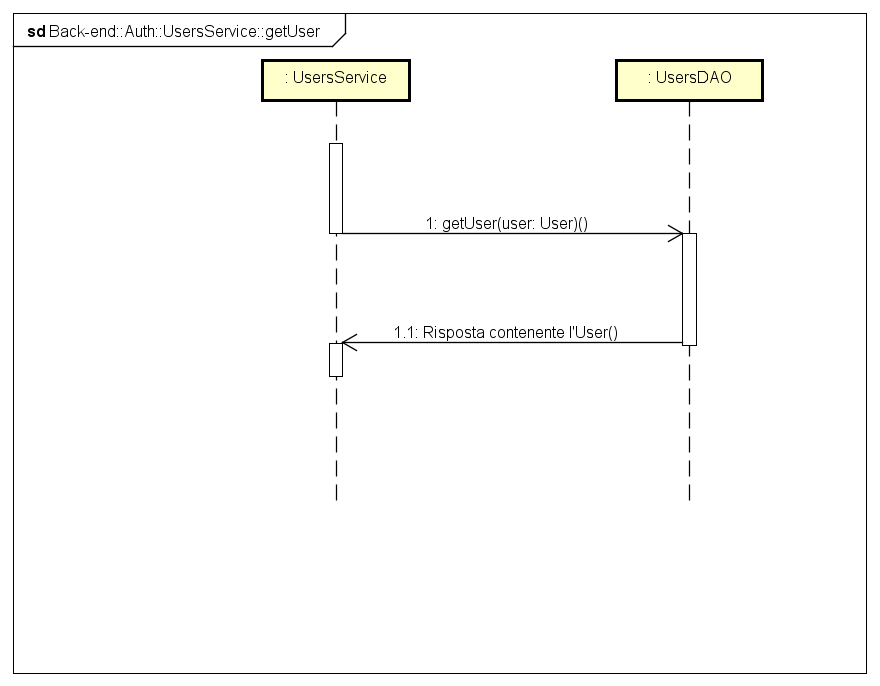
\includegraphics[width=\textwidth,height=\textheight,keepaspectratio]{images/diagrams/back-end/Ufficial_Backend/Back-endAuthUsersServicegetUser.png} 	\caption{Back-end::Auth::UsersService::getUser}
\end{figure} 
\newpage

\subsection{Back-end::Auth::UsersService::getUserList}
Il diagramma qui riportato rappresenta l'implementazione della lambda function che si occupa di ottenere la lista degli \file{User} del sistema attraverso il metodo \file{getUserList}.
\begin{figure}[h] \centering 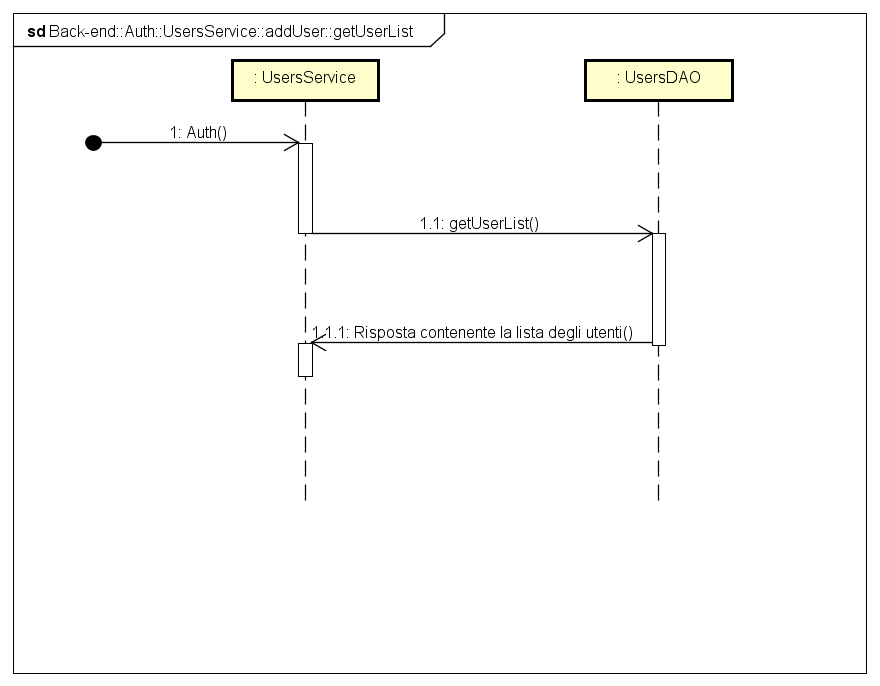
\includegraphics[width=\textwidth,height=\textheight,keepaspectratio]{images/diagrams/back-end/Ufficial_Backend/Back-endAuthUsersServicegetUserList.png} 	\caption{Back-end::Auth::UsersService::getUserList}
\end{figure}
\newpage

\subsection{Back-end::Auth::UsersService::removeUser}
Il diagramma qui riportato rappresenta l'implementazione della lambda function che si occupa di rimuovere un \file{User} dal sistema attraverso il metodo \file{removeUser}.
\begin{figure}[h] \centering 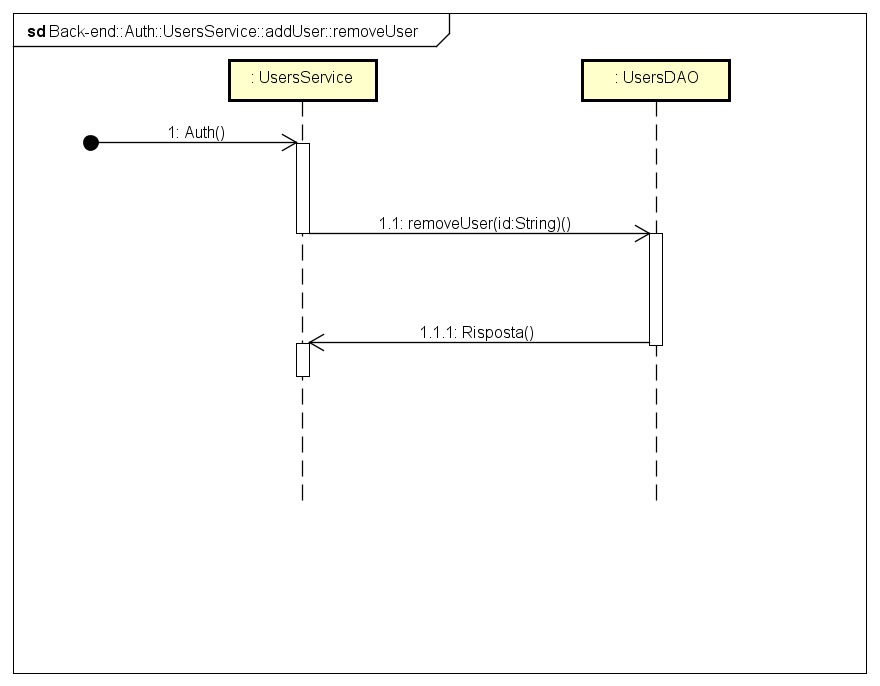
\includegraphics[width=\textwidth,height=\textheight,keepaspectratio]{images/diagrams/back-end/Ufficial_Backend/Back-endAuthUsersServiceremoveUser.png} 	\caption{Back-end::Auth::UsersService::removeUser}
\end{figure} 
\newpage

\subsection{Back-end::Auth::UsersService::updateUser}
Il diagramma qui riportato rappresenta l'implementazione della lambda function che si occupa di modificare un \file{User} del sistema attraverso il metodo \file{updateUser}.
\begin{figure}[h] \centering 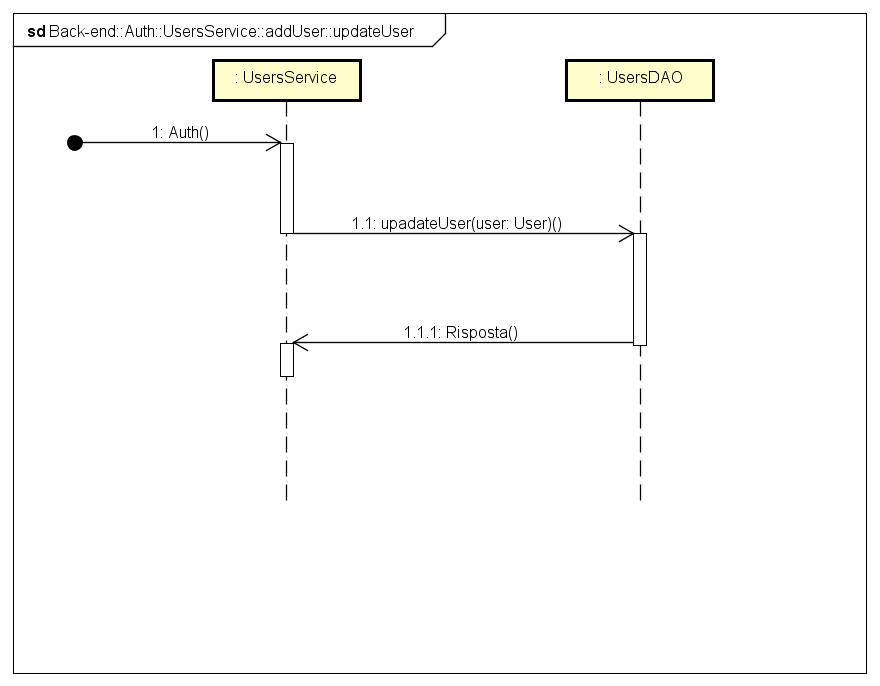
\includegraphics[width=\textwidth,height=\textheight,keepaspectratio]{images/diagrams/back-end/Ufficial_Backend/Back-endAuthUsersServiceupdateUser.png} 	\caption{Back-end::Auth::UsersService::updateUser}
\end{figure}
\newpage

\subsection{Back-end::Auth::UsersDAO\gl{DynamoDB}addUser}
Il diagramma qui riportato rappresenta l'aggiunta di un \file{User} al database attraverso il metodo \file{put} del \file{DocumentClient} di \file{DynamoDB}, utilizzando la risposta come parametro per chiamare la funzione di \gl{callback}.
\begin{figure}[h] \centering 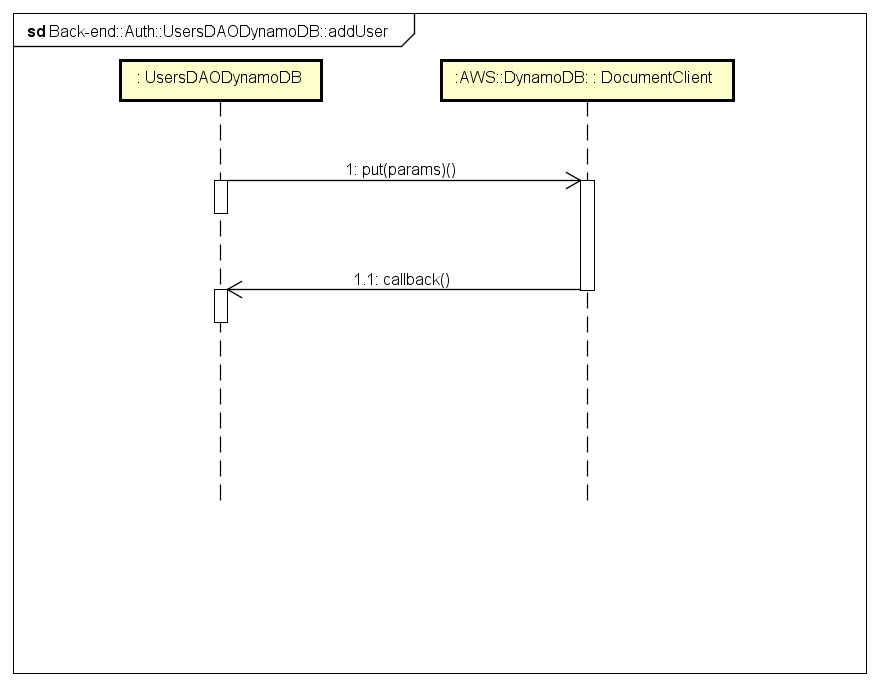
\includegraphics[width=\textwidth,height=\textheight,keepaspectratio]{images/diagrams/back-end/Ufficial_Backend/Back-endAuthUsersDAODynamoDBaddUser.png} 	\caption{Back-end::Auth::UsersDAODynamoDBaddUser}
\end{figure} 
\newpage
\subsection{Back-end::Auth::UsersDAODynamoDBgetUser}
Il diagramma qui riportato rappresenta l'ottenimento di un \file{User} dal database attraverso il metodo \file{get} del \file{DocumentClient} di \file{DynamoDB}, utilizzando la risposta come parametro per chiamare la funzione di callback.
\begin{figure}[h] \centering 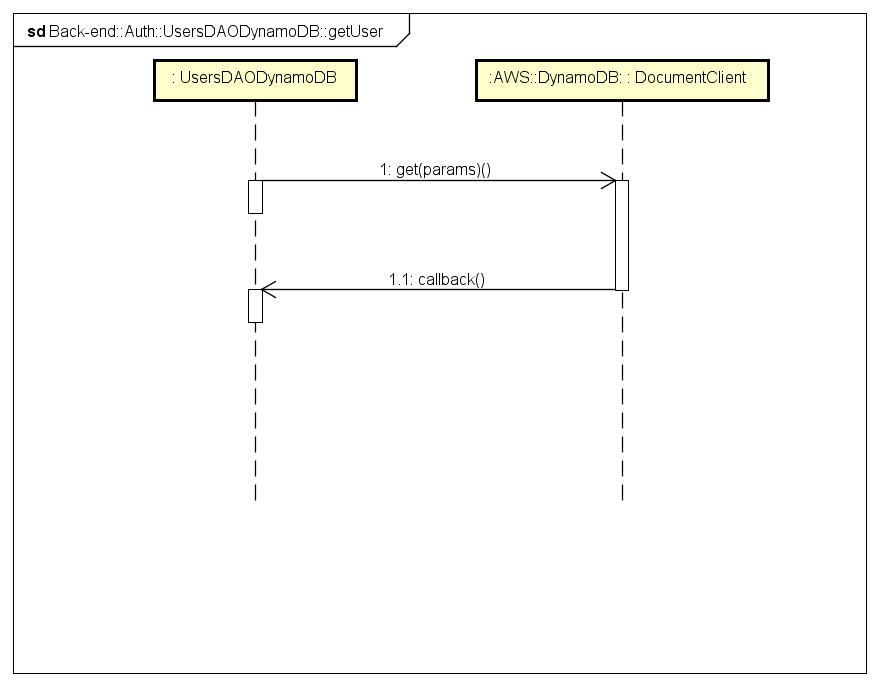
\includegraphics[width=\textwidth,height=\textheight,keepaspectratio]{images/diagrams/back-end/Ufficial_Backend/Back-endAuthUsersDAODynamoDBgetUser.png} 	\caption{Back-end::Auth::UsersDAODynamoDBgetUser}
\end{figure} 
\newpage
\subsection{Back-end::Auth::UsersDAODynamoDBgetUserList}
Il diagramma qui riportato rappresenta l'ottenimento della lista di \file{User} dal database attraverso il metodo \file{scan} del \file{DocumentClient} di \file{DynamoDB}, utilizzando la risposta come parametro per chiamare la funzione di callback. Poichè il metodo \file{scan} del \file{DocumentClient} permette al più il ritorno di una lista delle dimensioni di 1MB, se il campo LastEvaluetedKey è settato allora non tutti gli \file{User} sono stati ritornati, e quindi è necessario rieseguire il metodo scan fornendo come parametro d'ingresso la chiave da cui ripartire per l'estrazione dei dati. Se invece tale campo non è settato allora è stata ritornata l'intera lista.
\begin{figure}[h] \centering 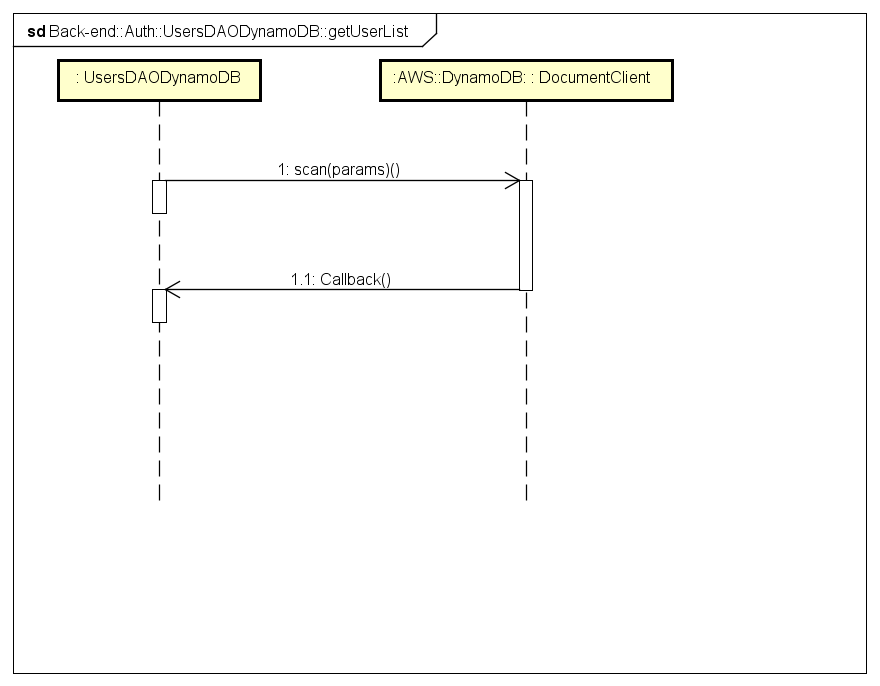
\includegraphics[width=\textwidth,height=\textheight,keepaspectratio]{images/diagrams/back-end/Ufficial_Backend/Back-endAuthUsersDAODynamoDBgetUserList.png} 	\caption{Back-end::Auth::UsersDAODynamoDBgetUserList}
\end{figure}
\newpage

\subsection{Back-end::Auth::UsersDAODynamoDB::removeUser}
Il diagramma qui riportato rappresenta la rimozione di un \file{User} dal database attraverso il metodo \file{delete} del \file{DocumentClient} di \file{DynamoDB}, utilizzando la risposta come parametro per chiamare la funzione di callback.
 \begin{figure}[h] \centering 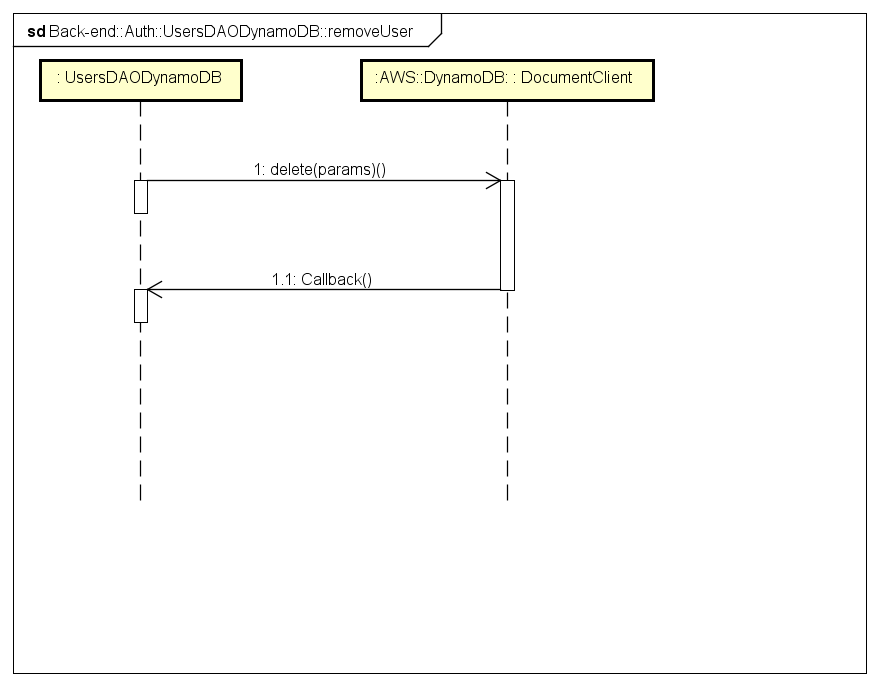
\includegraphics[width=\textwidth,height=\textheight,keepaspectratio]{images/diagrams/back-end/Ufficial_Backend/Back-endAuthUsersDAODynamoDBremoveUser.png} 	\caption{Back-end::Auth::UsersDAODynamoDB::removeUser}
\end{figure} 
\newpage

\subsection{Back-end::Auth::UsersDAODynamoDB::updateUser}
Il diagramma qui riportato rappresenta la modifica di un \file{User} del database attraverso il metodo \file{update} del \file{DocumentClient} di \file{DynamoDB}, utilizzando la risposta come parametro per chiamare la funzione di callback.
\begin{figure}[h] \centering 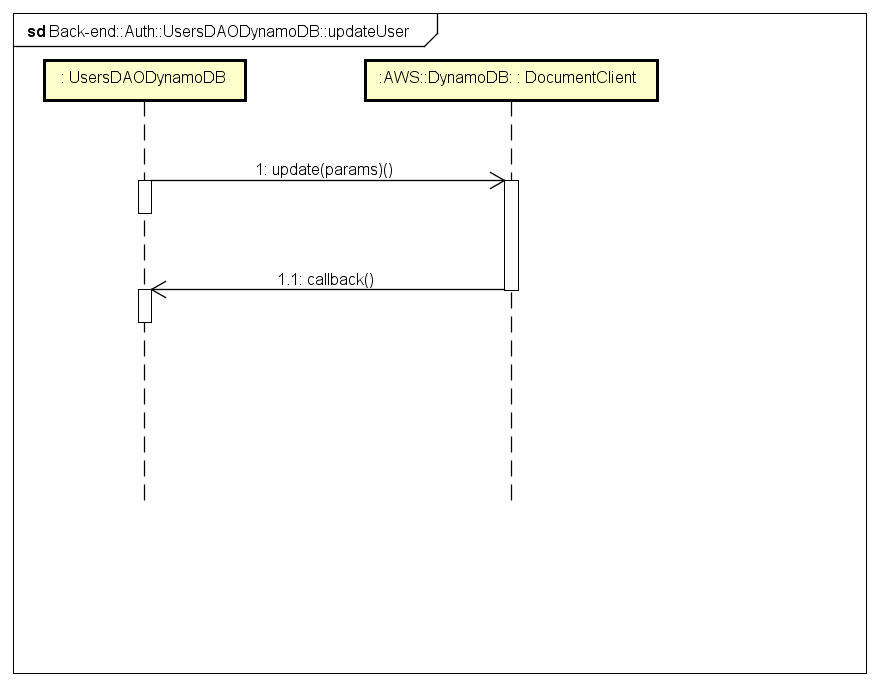
\includegraphics[width=\textwidth,height=\textheight,keepaspectratio]{images/diagrams/back-end/Ufficial_Backend/Back-endAuthUsersDAODynamoDBupdateUser.png} 	\caption{Back-end::Auth::UsersDAODynamoDB::updateUser}
\end{figure}
\newpage


\subsection{Back-end::ConversationsDAODynamoDB::addConversation}
Il diagramma qui riportato rappresenta l'aggiunta di una \file{Conversation} al database attraverso il metodo \file{put} del \file{DocumentClient} di \file{DynamoDB}, utilizzando la risposta come parametro per chiamare la funzione di callback.
 \begin{figure}[h] \centering 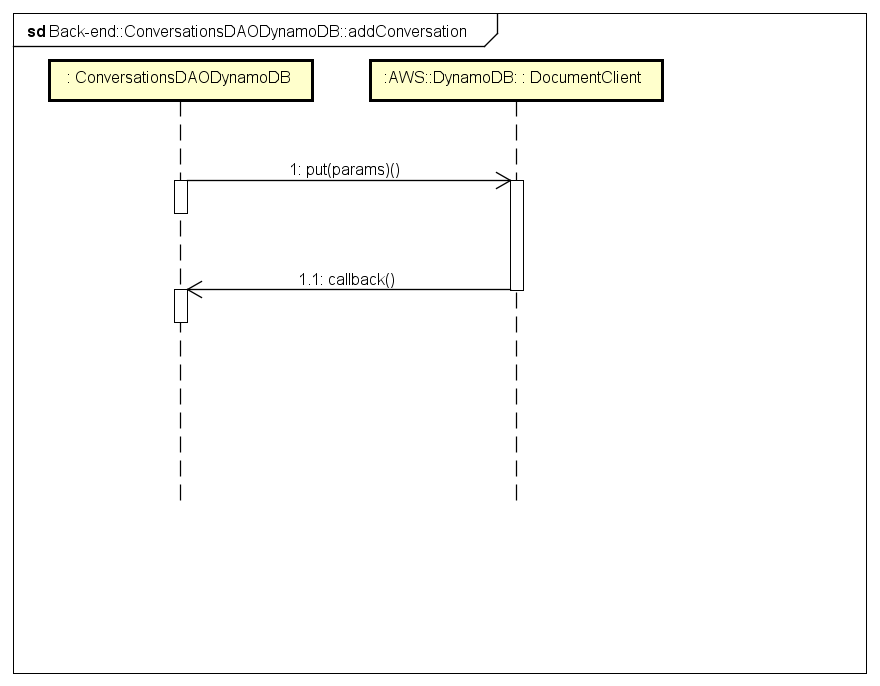
\includegraphics[width=\textwidth,height=\textheight,keepaspectratio]{images/diagrams/back-end/Ufficial_Backend/Back-endConversationsDAODynamoDBaddConversation.png} 	\caption{Back-end::ConversationsDAODynamoDB::addConversation}
\end{figure}
\newpage

\subsection{Back-end::ConversationsDAODynamoDB::addMessage}
Il diagramma qui riportato rappresenta l'aggiunta di un \file{Message} al database attraverso il metodo \file{put} del \file{DocumentClient} di \file{DynamoDB}, utilizzando la risposta come parametro per chiamare la funzione di callback.
 \begin{figure}[h] \centering 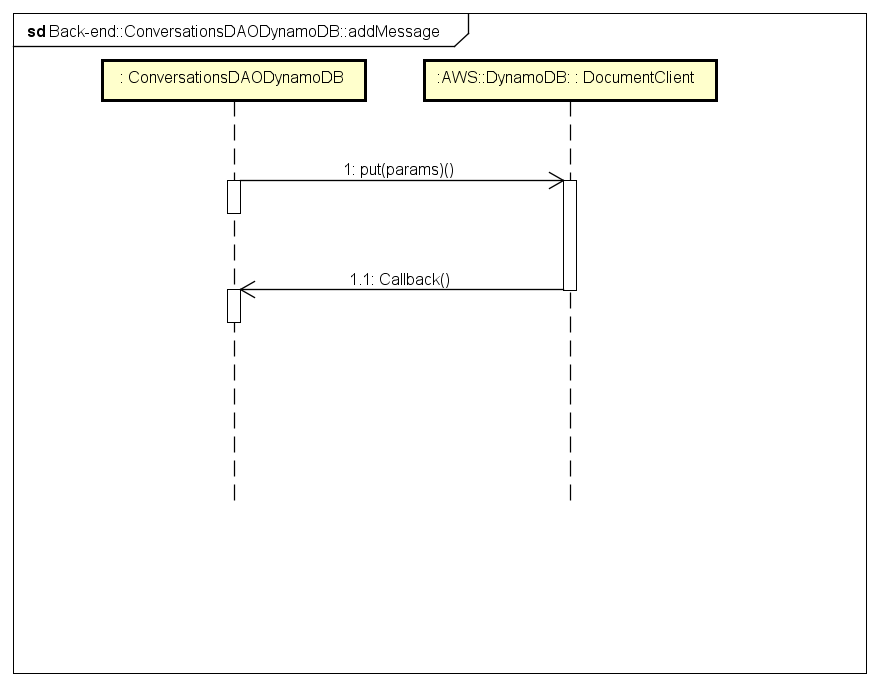
\includegraphics[width=\textwidth,height=\textheight,keepaspectratio]{images/diagrams/back-end/Ufficial_Backend/Back-endConversationsDAODynamoDBaddMessage.png} 	\caption{Back-end::ConversationsDAODynamoDB::addMessage}
\end{figure}
\newpage

\subsection{Back-end::ConversationsDAODynamoDB::getConversation}
Il diagramma qui riportato rappresenta l'ottenimento di una \file{Conversation} dal database attraverso il metodo \file{get} del \file{DocumentClient} di \file{DynamoDB}, utilizzando la risposta come parametro per chiamare la funzione di callback.
 \begin{figure}[h] \centering 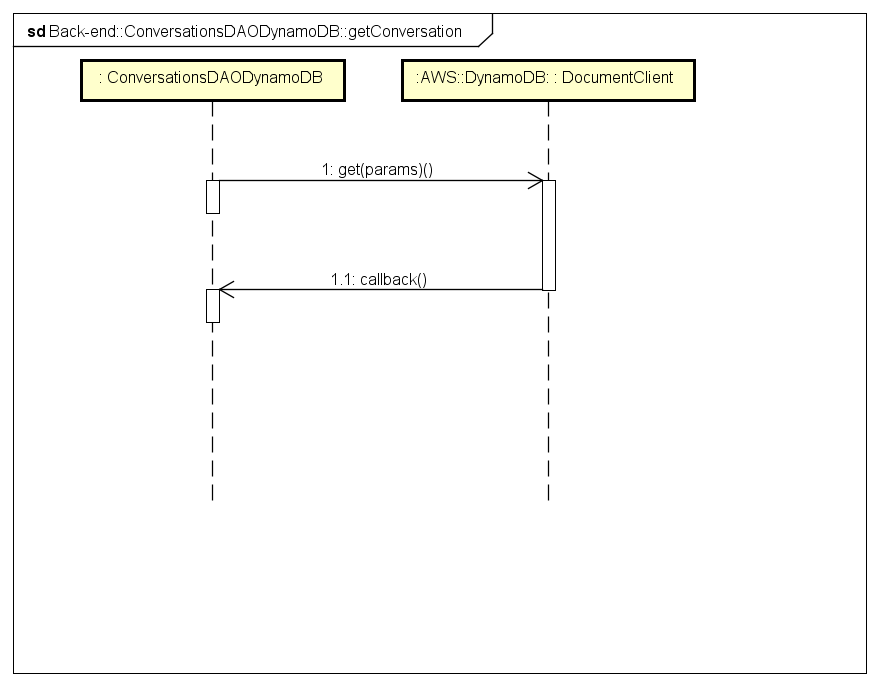
\includegraphics[width=\textwidth,height=\textheight,keepaspectratio]{images/diagrams/back-end/Ufficial_Backend/Back-endConversationsDAODynamoDBgetConversation.png} 	\caption{Back-end::ConversationsDAODynamoDB::getConversation}
\end{figure}
\newpage

\subsection{Back-end::ConversationsDAODynamoDB::getConversationList}
Il diagramma qui riportato rappresenta l'ottenimento della lista di \file{Conversation} dal database attraverso il metodo \file{scan} del \file{DocumentClient} di \file{DynamoDB}, utilizzando la risposta come parametro per chiamare la funzione di callback. Poichè il metodo \file{scan} del \file{DocumentClient} permette al più il ritorno di una lista delle dimensioni di 1MB, se il campo LastEvaluetedKey è settato allora non tutti le \file{Conversation} sono state ritornate, e quindi è necessario rieseguire il metodo scan fornendo come parametro d'ingresso la chiave da cui ripartire per l'estrazione dei dati. Se invece tale campo non è settato allora è stata ritornata l'intera lista.
 \begin{figure}[h] \centering 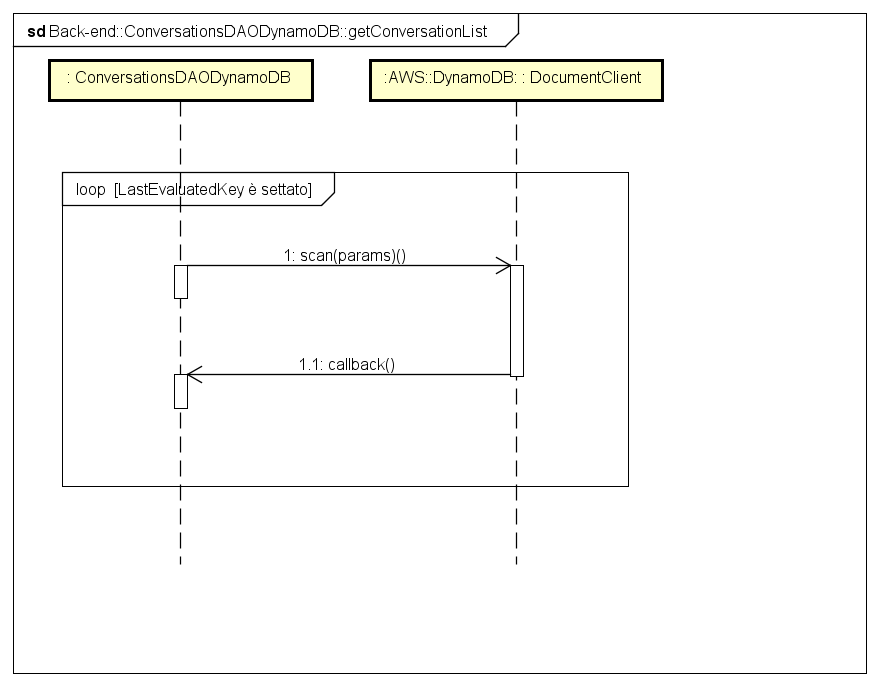
\includegraphics[width=\textwidth,height=\textheight,keepaspectratio]{images/diagrams/back-end/Ufficial_Backend/Back-endConversationsDAODynamoDBgetConversationList.png} 	\caption{Back-end::ConversationsDAODynamoDB::getConversationList}
\end{figure}
\newpage

\subsection{Back-end::ConversationsDAODynamoDB::removeConversation} 
Il diagramma qui riportato rappresenta la rimozione di una \file{Conversation} dal database attraverso il metodo \file{delete} del \file{DocumentClient} di \file{DynamoDB}, utilizzando la risposta come parametro per chiamare la funzione di callback.
\begin{figure}[h] \centering 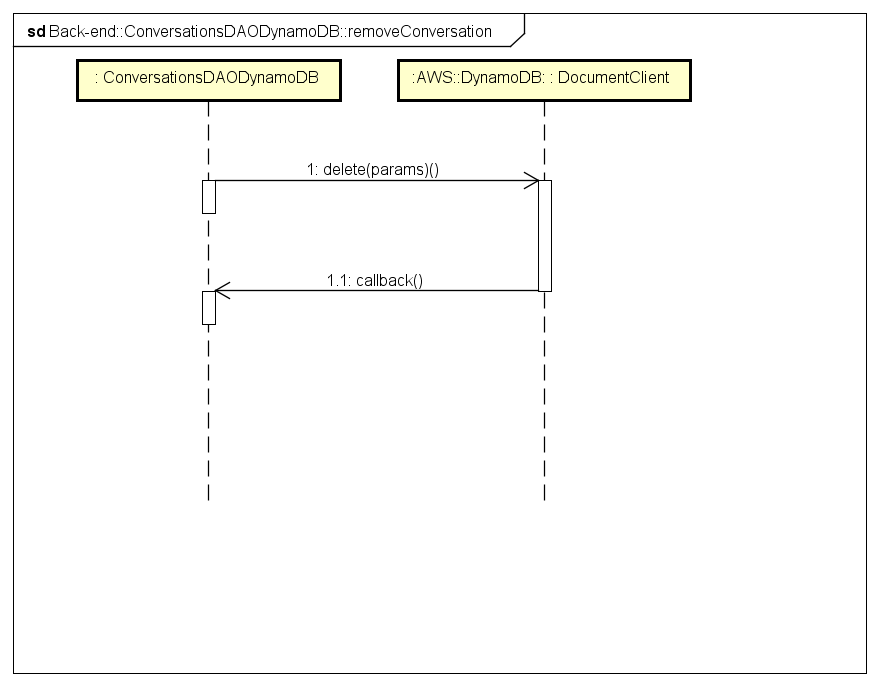
\includegraphics[width=\textwidth,height=\textheight,keepaspectratio]{images/diagrams/back-end/Ufficial_Backend/Back-endConversationsDAODynamoDBremoveConversation.png} 	\caption{Back-end::ConversationsDAODynamoDB::removeConversation}
\end{figure}

\newpage

\subsection{Back-end::GuestsDAODynamoDB::addGuest}
Il diagramma qui riportato rappresenta l'aggiunta di un \file{Guest} al database attraverso il metodo \file{add} del \file{DocumentClient} di \file{DynamoDB}, utilizzando la risposta come parametro per chiamare la funzione di callback.
\begin{figure}[h] \centering 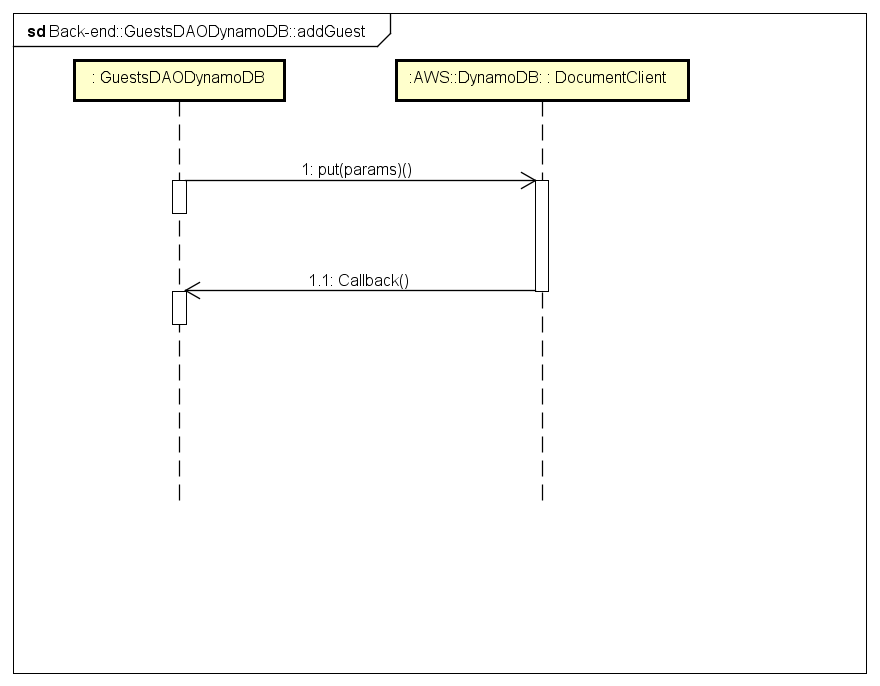
\includegraphics[width=\textwidth,height=\textheight,keepaspectratio]{images/diagrams/back-end/Ufficial_Backend/Back-endGuestsDAODynamoDBaddGuest.png} 	\caption{Back-end::GuestsDAODynamoDB::addGuest}
\end{figure}
\newpage

\subsection{Back-end::ConversationsDAODynamoDB::getGuest}
Il diagramma qui riportato rappresenta l'ottenimento di un \file{Guest} dal database attraverso il metodo \file{get} del \file{DocumentClient} di \file{DynamoDB}, utilizzando la risposta come parametro per chiamare la funzione di callback.
 \begin{figure}[h] \centering 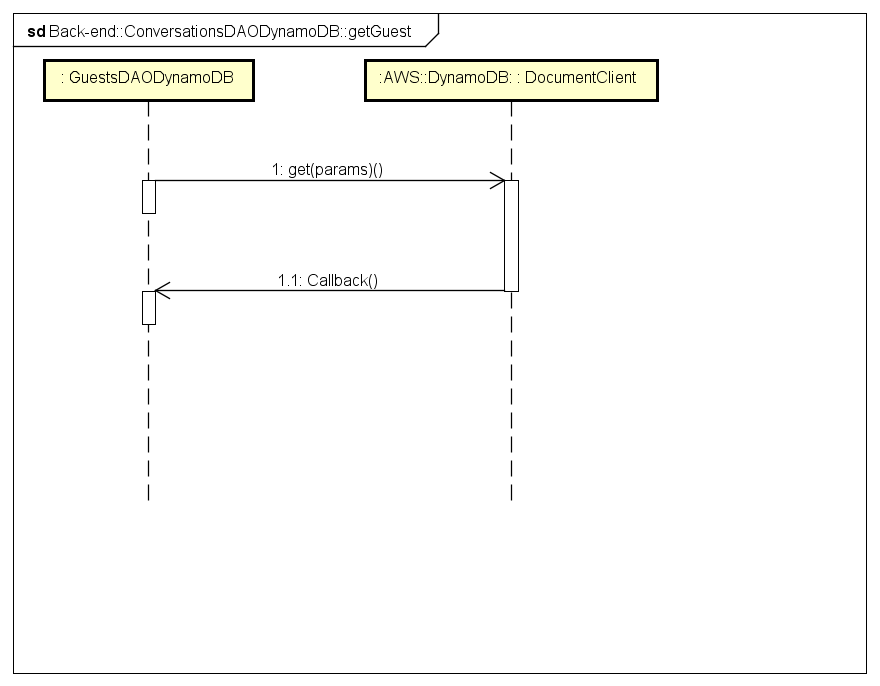
\includegraphics[width=\textwidth,height=\textheight,keepaspectratio]{images/diagrams/back-end/Ufficial_Backend/Back-endConversationsDAODynamoDBgetGuest.png} 	\caption{Back-end::ConversationsDAODynamoDB::getGuest}
\end{figure}
\newpage

\subsection{Back-end::ConversationsDAODynamoDB::getGuestList}
Il diagramma qui riportato rappresenta l'ottenimento della lista di \file{Guest} dal database attraverso il metodo \file{scan} del \file{DocumentClient} di \file{DynamoDB}, utilizzando la risposta come parametro per chiamare la funzione di callback. Poichè il metodo \file{scan} del \file{DocumentClient} permette al più il ritorno di una lista delle dimensioni di 1MB, se il campo LastEvaluetedKey è settato allora non tutti i \file{Guest} sono stati ritornati, e quindi è necessario rieseguire il metodo scan fornendo come parametro d'ingresso la chiave da cui ripartire per l'estrazione dei dati. Se invece tale campo non è settato allora è stata ritornata l'intera lista.
 \begin{figure}[h] \centering 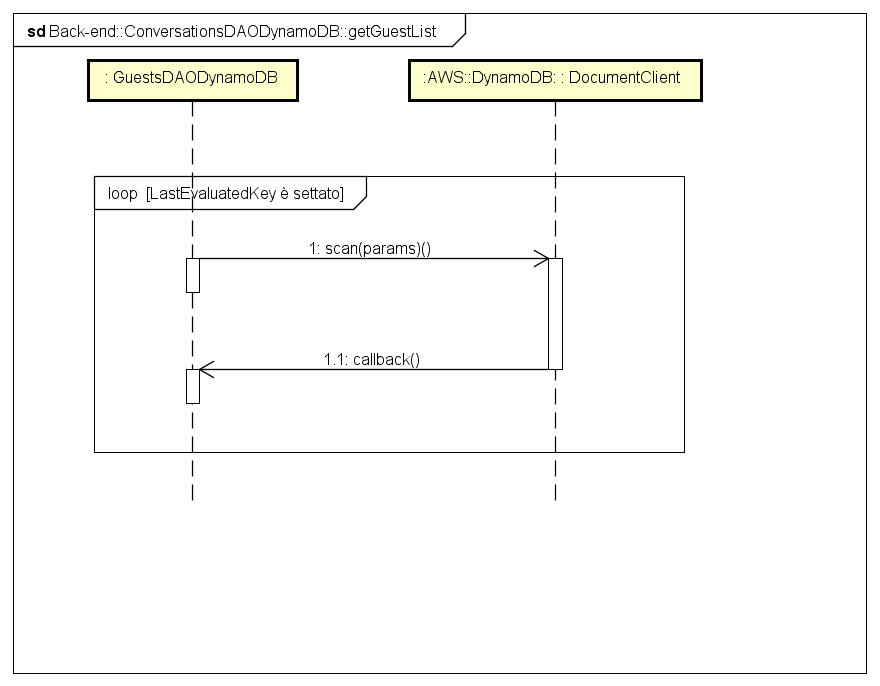
\includegraphics[width=\textwidth,height=\textheight,keepaspectratio]{images/diagrams/back-end/Ufficial_Backend/Back-endConversationsDAODynamoDBgetGuestList.png} 	\caption{Back-end::ConversationsDAODynamoDB::getGuestList}
\end{figure}

\newpage



\subsection{Back-end::ConversationsDAODynamoDB::removeGuest}
Il diagramma qui riportato rappresenta la rimozione di un \file{Guest} dal database attraverso il metodo \file{delete} del \file{DocumentClient} di \file{DynamoDB}, utilizzando la risposta come parametro per chiamare la funzione di callback.
 \begin{figure}[h] \centering 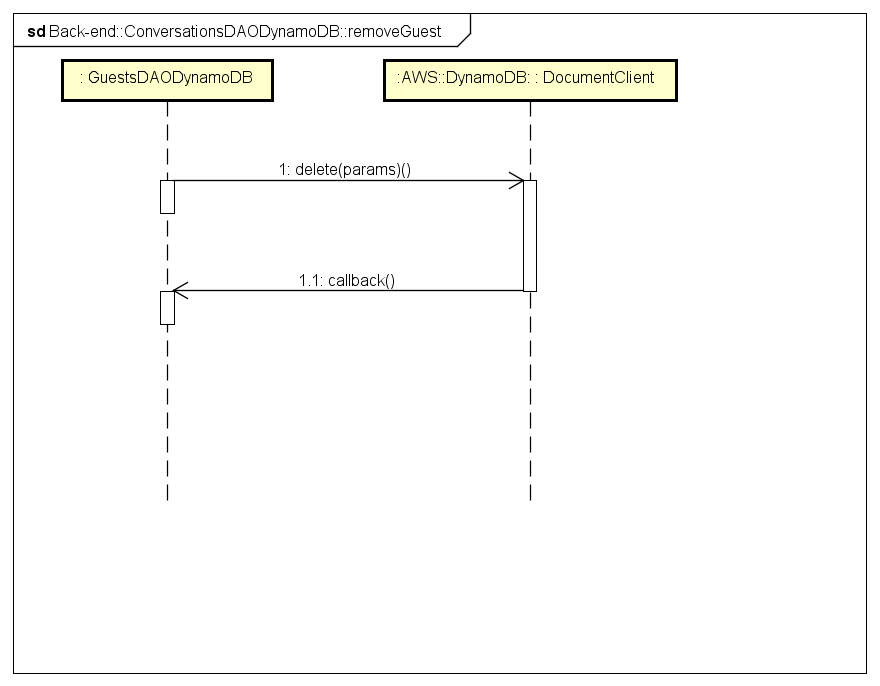
\includegraphics[width=\textwidth,height=\textheight,keepaspectratio]{images/diagrams/back-end/Ufficial_Backend/Back-endConversationsDAODynamoDBremoveGuest.png} 	\caption{Back-end::ConversationsDAODynamoDB::removeGuest}
\end{figure}

\newpage

\subsection{Back-end::ConversationsDAODynamoDB::updateGuest}
Il diagramma qui riportato rappresenta la modifica di un \file{Guest} del database attraverso il metodo \file{update} del \file{DocumentClient} di \file{DynamoDB}, utilizzando la risposta come parametro per chiamare la funzione di callback.
 \begin{figure}[h] \centering 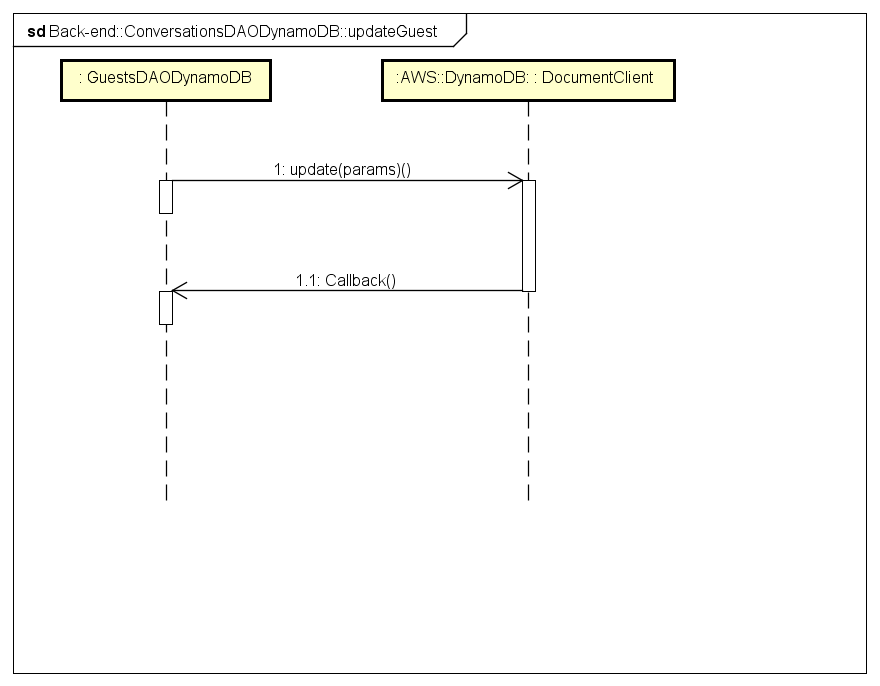
\includegraphics[width=\textwidth,height=\textheight,keepaspectratio]{images/diagrams/back-end/Ufficial_Backend/Back-endConversationsDAODynamoDBupdateGuest.png} 	\caption{Back-end::ConversationsDAODynamoDB::updateGuest}
\end{figure} 
\newpage


\subsection{Back-end::Notifications::NotificationService::getChannelList}
Il diagramma qui riportato rappresenta la richiesta dei canali disponibili al servizio esterno \file{\gl{Slack}}, utilizzando il metodo \file{channels.list} messo a disposizione da \file{Slack}.
 \begin{figure}[h] \centering 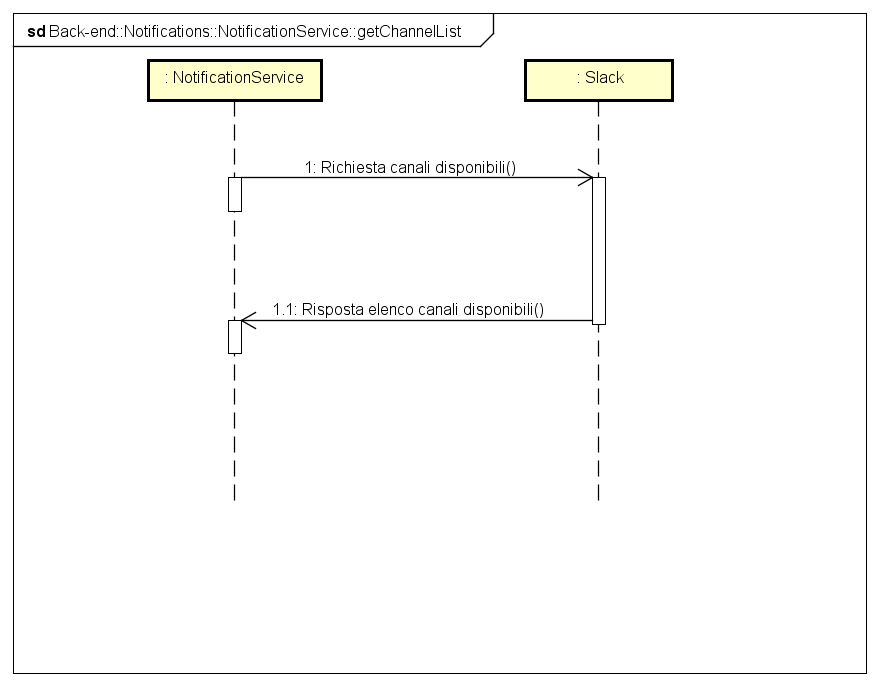
\includegraphics[width=\textwidth,height=\textheight,keepaspectratio]{images/diagrams/back-end/Ufficial_Backend/Back-endNotificationsNotificationServicegetChannelList.png} 	\caption{Back-end::Notifications::NotificationService::getChannelList}
\end{figure}

\subsection{Back-end::Notifications::NotificationService::sendMsg}
Il diagramma qui riportato rappresenta l'invio di un messaggio al servizio esterno \file{Slack}.
 \begin{figure}[h] \centering 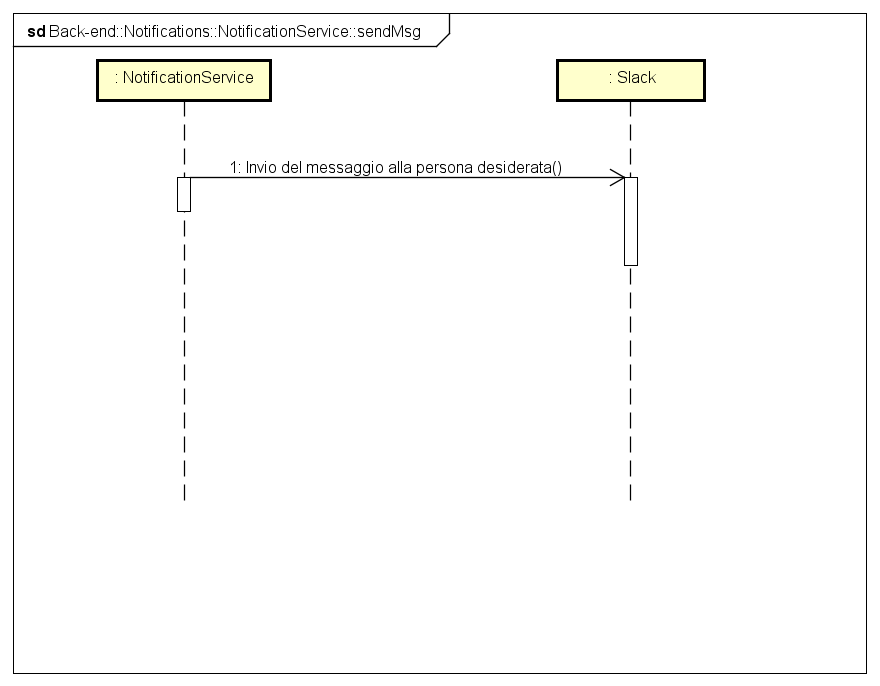
\includegraphics[width=\textwidth,height=\textheight,keepaspectratio]{images/diagrams/back-end/Ufficial_Backend/Back-endNotificationsNotificationServicesendMsg.png} 	\caption{Back-end::Notifications::NotificationService::sendMsg} 
\end{figure}

\newpage


\subsection{Back-end::\gl{Rule}s::RulesService::addRule}
Il diagramma qui riportato rappresenta l'implementazione della lambda function che si occupa di aggiungere una \file{Rule} al sistema attraverso il metodo \file{addRule}. 
 \begin{figure}[h] \centering 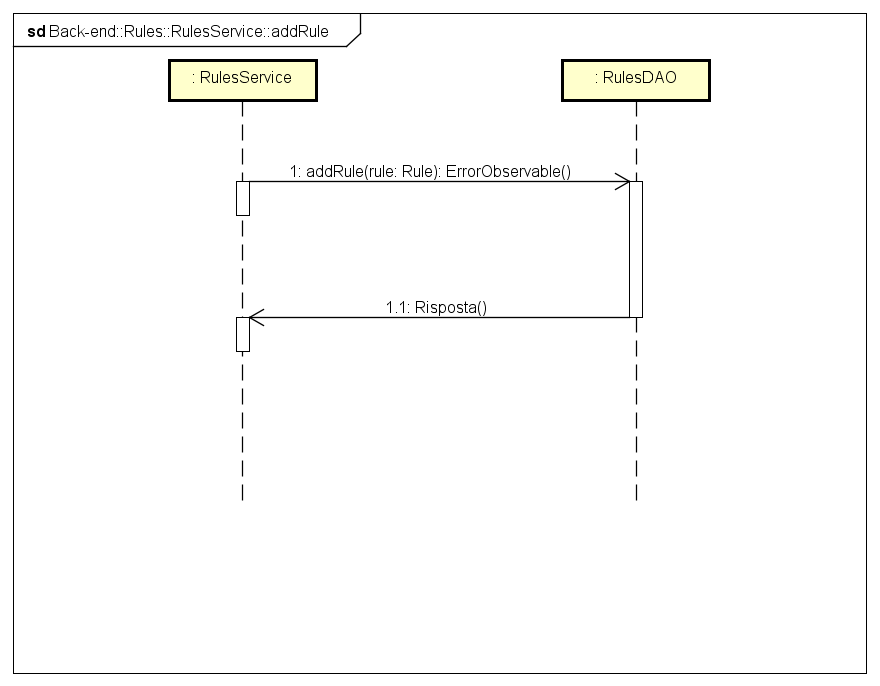
\includegraphics[width=\textwidth,height=\textheight,keepaspectratio]{images/diagrams/back-end/Ufficial_Backend/Back-endRulesRulesServiceaddRule.png} 	\caption{Back-end::Rules::RulesService::addRule}
\end{figure} 
\newpage



\subsection{Back-end::Rules::RulesService::getFunction}
Il diagramma qui riportato rappresenta l'implementazione della lambda function che si occupa di ottenere una \file{Function} del sistema attraverso il metodo \file{getFunction}. 
 \begin{figure}[h] \centering 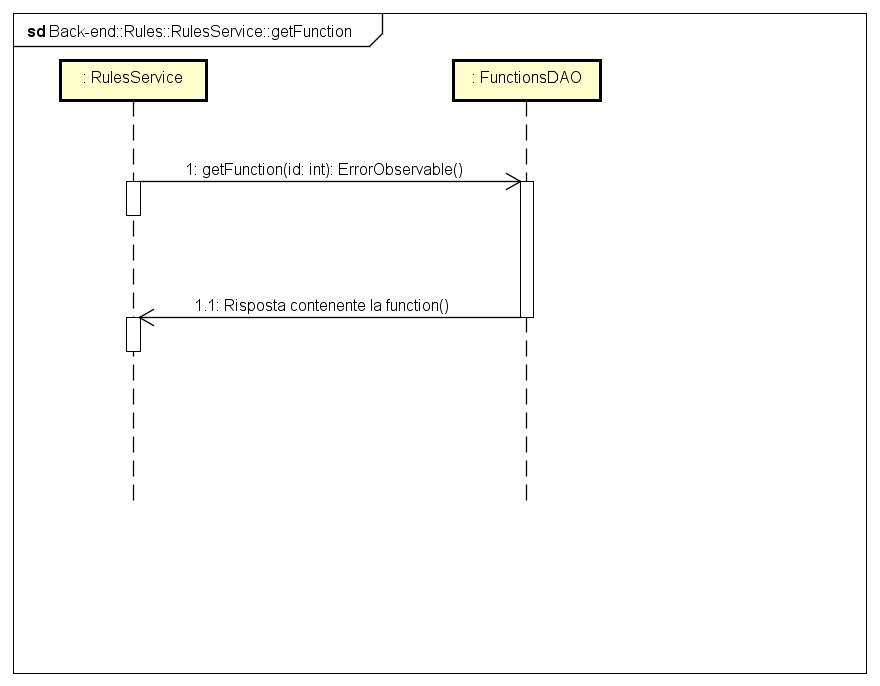
\includegraphics[width=\textwidth,height=\textheight,keepaspectratio]{images/diagrams/back-end/Ufficial_Backend/Back-endRulesRulesServicegetFunction.png} 	\caption{Back-end::Rules::RulesService::getFunction}
\end{figure}
\newpage

\subsection{Back-end::Rules::RulesService::getFunctionList}
Il diagramma qui riportato rappresenta l'implementazione della lambda function che si occupa di ottenere la lista delle \file{Function} del sistema attraverso il metodo \file{getFunctionList}.
 \begin{figure}[h] \centering 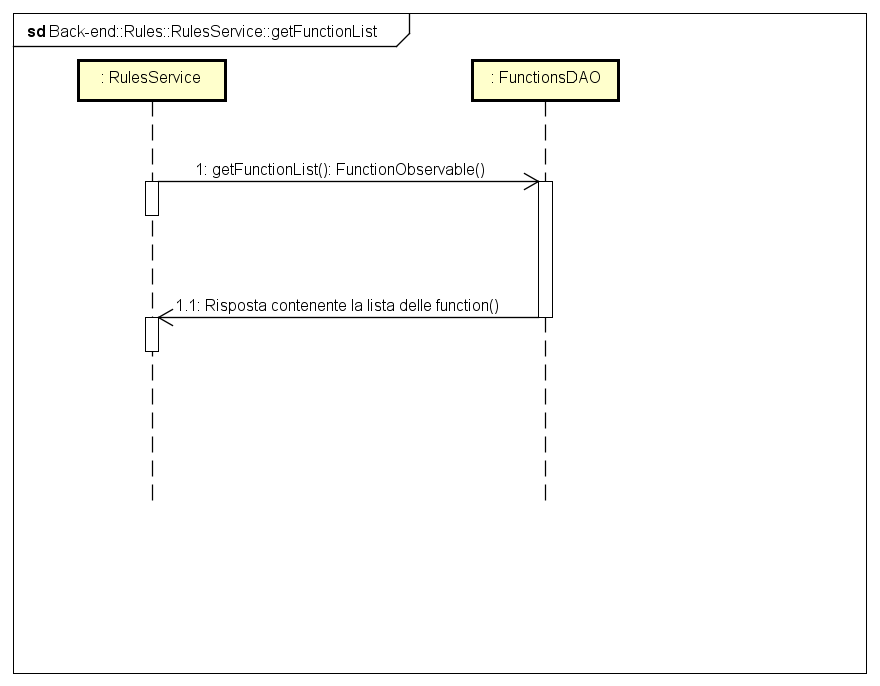
\includegraphics[width=\textwidth,height=\textheight,keepaspectratio]{images/diagrams/back-end/Ufficial_Backend/Back-endRulesRulesServicegetFunctionList.png} 	\caption{Back-end::Rules::RulesService::getFunctionList}
\end{figure} 
\newpage

\subsection{Back-end::Rules::RulesService::getRule}
Il diagramma qui riportato rappresenta l'implementazione della lambda function che si occupa di ottenere una \file{Rule} del sistema attraverso il metodo \file{getRule}. 
\begin{figure}[h] \centering 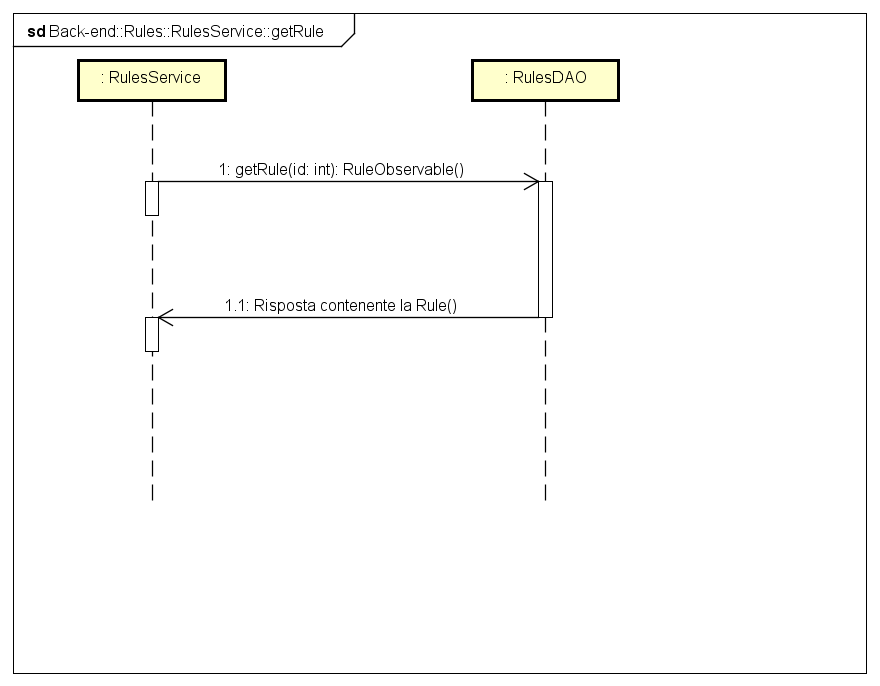
\includegraphics[width=\textwidth,height=\textheight,keepaspectratio]{images/diagrams/back-end/Ufficial_Backend/Back-endRulesRulesServicegetRule.png} 	\caption{Back-end::Rules::RulesService::getRule}
\end{figure} 
\newpage

\subsection{Back-end::Rules::RulesService::getRuleList}
Il diagramma qui riportato rappresenta l'implementazione della lambda function che si occupa di ottenere la lista delle \file{Rule} del sistema attraverso il metodo \file{getRuleList}.
\begin{figure}[h] \centering 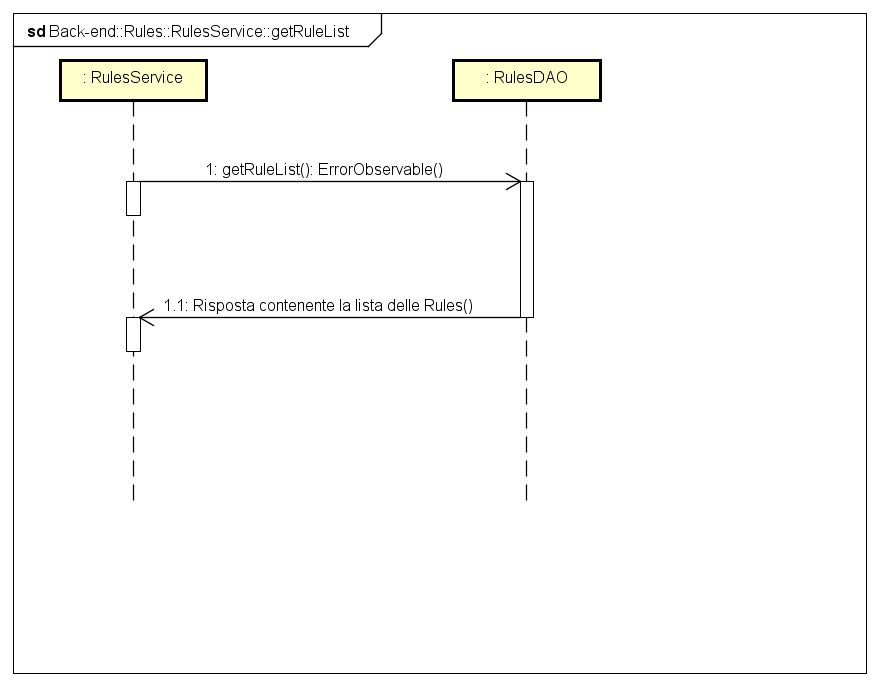
\includegraphics[width=\textwidth,height=\textheight,keepaspectratio]{images/diagrams/back-end/Ufficial_Backend/Back-endRulesRulesServicegetRuleList.png} 	\caption{Back-end::Rules::RulesService::getRuleList}
\end{figure} 
\newpage

\subsection{Back-end::Rules::RulesService::deleteRule}
Il diagramma qui riportato rappresenta l'implementazione della lambda function che si occupa di rimuovere una \file{Rule} dal sistema attraverso il metodo \file{deleteRule}. 
\begin{figure}[h] \centering 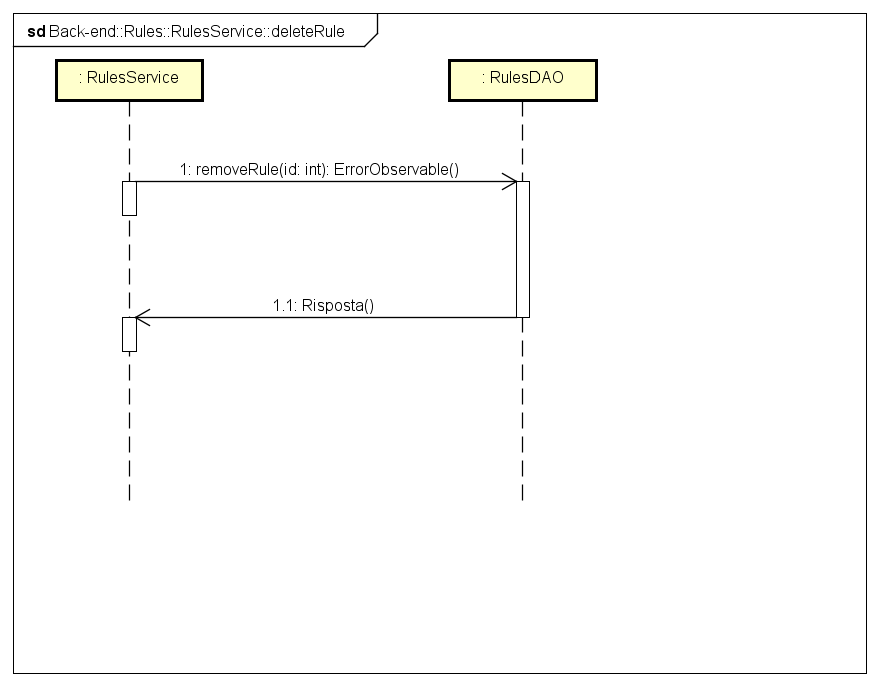
\includegraphics[width=\textwidth,height=\textheight,keepaspectratio]{images/diagrams/back-end/Ufficial_Backend/Back-endRulesRulesServicedeleteRule.png} 	\caption{Back-end::Rules::RulesService::deleteRule}
\end{figure}
\newpage

\subsection{Back-end::Rules::RulesService::updateRule}
Il diagramma qui riportato rappresenta l'implementazione della lambda function che si occupa di modificare una \file{Rule} del sistema attraverso il metodo \file{updateRule}.
\begin{figure}[h] \centering 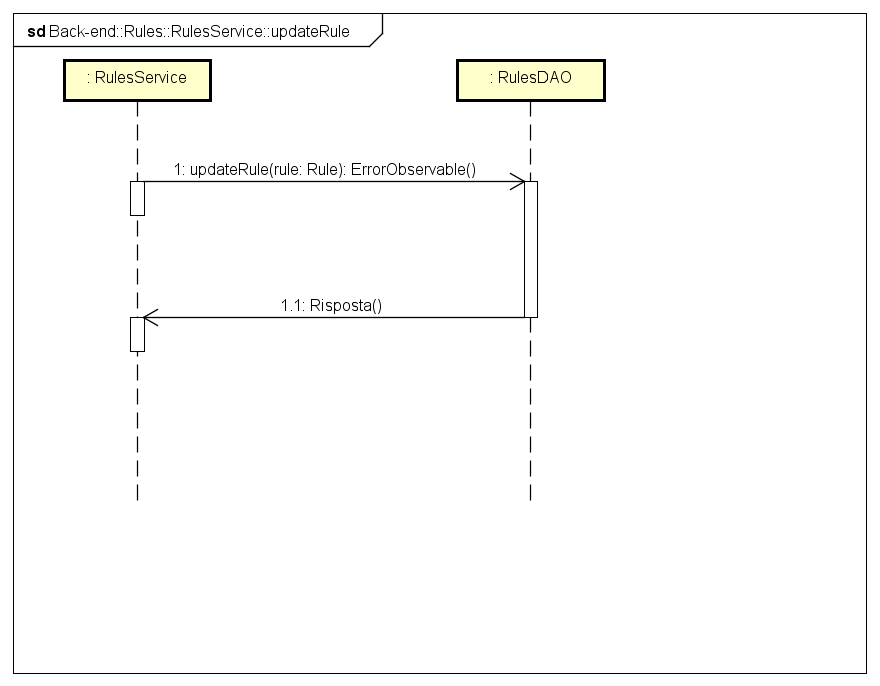
\includegraphics[width=\textwidth,height=\textheight,keepaspectratio]{images/diagrams/back-end/Ufficial_Backend/Back-endRulesRulesServiceupdateRule.png} 	\caption{Back-end::Rules::RulesService::updateRule}
\end{figure} 
\newpage


\subsection{Back-end::Rules::FunctionsDAODynamoDB::addFunction}
Il diagramma qui riportato rappresenta l'aggiunta di una \file{Function} al database attraverso il metodo \file{put} del \file{DocumentClient} di \file{DynamoDB}, utilizzando la risposta come parametro per chiamare la funzione di callback.
 \begin{figure}[h] \centering 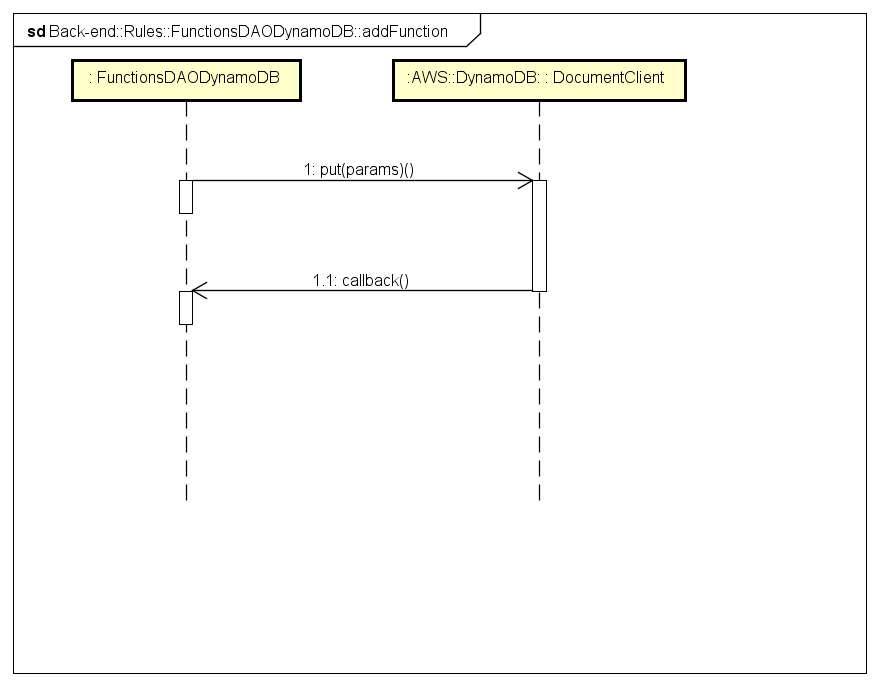
\includegraphics[width=\textwidth,height=\textheight,keepaspectratio]{images/diagrams/back-end/Ufficial_Backend/Back-endRulesFunctionsDAODynamoDBaddFunction.png} 	\caption{Back-end::Rules::FunctionsDAODynamoDB::addFunction}
\end{figure}

\newpage
\subsection{Back-end::Rules::FunctionsDAODynamoDB::getFunction}
Il diagramma qui riportato rappresenta l'ottenimento di una \file{Function} dal database attraverso il metodo \file{get} del \file{DocumentClient} di \file{DynamoDB}, utilizzando la risposta come parametro per chiamare la funzione di callback. 
\begin{figure}[h] \centering 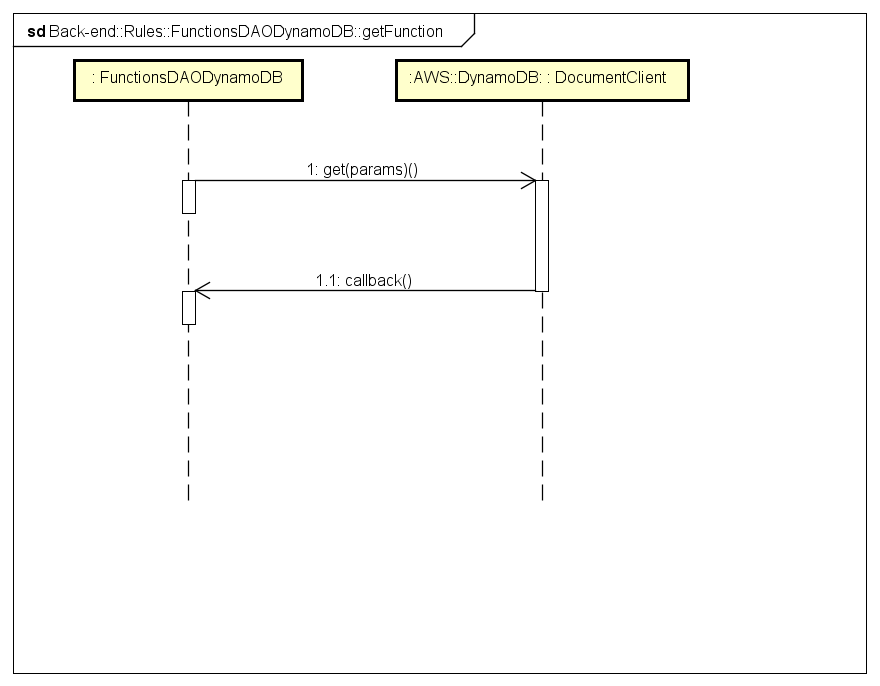
\includegraphics[width=\textwidth,height=\textheight,keepaspectratio]{images/diagrams/back-end/Ufficial_Backend/Back-endRulesFunctionsDAODynamoDBgetFunction.png} 	\caption{Back-end::Rules::FunctionsDAODynamoDB::getFunction}
\end{figure}
\newpage

\subsection{Back-end::Rules::FunctionsDAODynamoDB::getFunctionList}
Il diagramma qui riportato rappresenta l'ottenimento della lista di \file{Function} dal database attraverso il metodo \file{scan} del \file{DocumentClient} di \file{DynamoDB}, utilizzando la risposta come parametro per chiamare la funzione di callback. Poichè il metodo \file{scan} del \file{DocumentClient} permette al più il ritorno di una lista delle dimensioni di 1MB, se il campo LastEvaluetedKey è settato allora non tutte le \file{Function} sono state ritornate, e quindi è necessario rieseguire il metodo scan fornendo come parametro d'ingresso la chiave da cui ripartire per l'estrazione dei dati. Se invece tale campo non è settato allora è stata ritornata l'intera lista.
 \begin{figure}[h] \centering 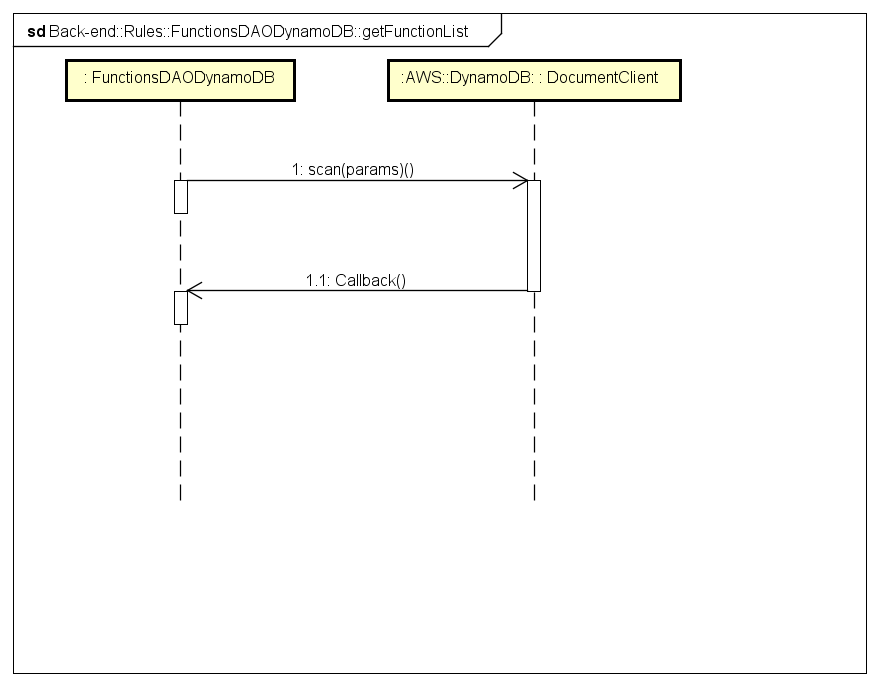
\includegraphics[width=\textwidth,height=\textheight,keepaspectratio]{images/diagrams/back-end/Ufficial_Backend/Back-endRulesFunctionsDAODynamoDBgetFunctionList.png} 	\caption{Back-end::Rules::FunctionsDAODynamoDB::getFunctionList}
\end{figure} 
\newpage

\subsection{Back-end::Rules::FunctionsDAODynamoDB::removeFunction}
Il diagramma qui riportato rappresenta la rimozione di una \file{Function} dal database attraverso il metodo \file{delete} del \file{DocumentClient} di \file{DynamoDB}, utilizzando la risposta come parametro per chiamare la funzione di callback. 
\begin{figure}[h] \centering 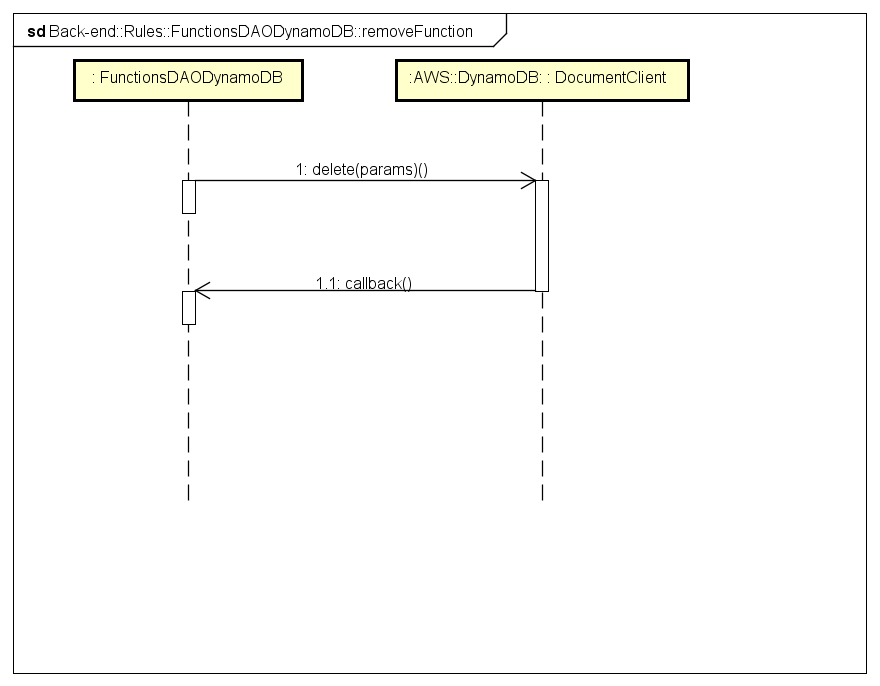
\includegraphics[width=\textwidth,height=\textheight,keepaspectratio]{images/diagrams/back-end/Ufficial_Backend/Back-endRulesFunctionsDAODynamoDBremoveFunction.png} 	\caption{Back-end::Rules::FunctionsDAODynamoDB::removeFunction}
\end{figure}
\newpage

\subsection{Back-end::Rules::FunctionsDAODynamoDB::updateFunction}
Il diagramma qui riportato rappresenta la modifica di una \file{Function} del database attraverso il metodo \file{update} del \file{DocumentClient} di \file{DynamoDB}, utilizzando la risposta come parametro per chiamare la funzione di callback. 
 \begin{figure}[h] \centering 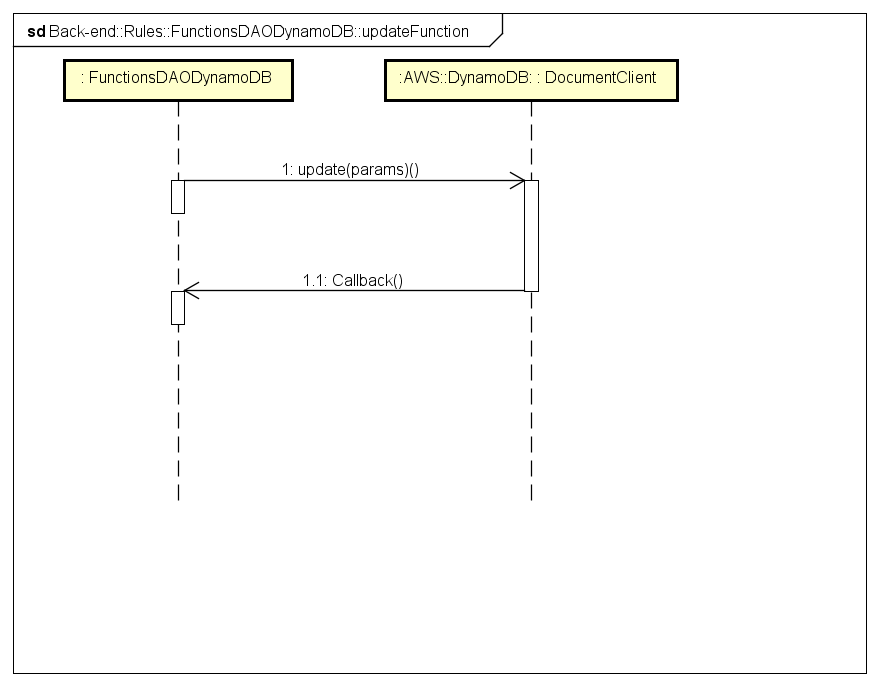
\includegraphics[width=\textwidth,height=\textheight,keepaspectratio]{images/diagrams/back-end/Ufficial_Backend/Back-endRulesFunctionsDAODynamoDBupdateFunction.png} 	\caption{Back-end::Rules::FunctionsDAODynamoDB::updateFunction}
\end{figure} 
\newpage

\subsection{Back-end::Rules::RulesDAODynamoDB::addRule}
Il diagramma qui riportato rappresenta l'aggiunta di una \file{Rule} al database attraverso il metodo \file{put} del \file{DocumentClient} di \file{DynamoDB}, utilizzando la risposta come parametro per chiamare la funzione di callback.
\begin{figure}[h] \centering 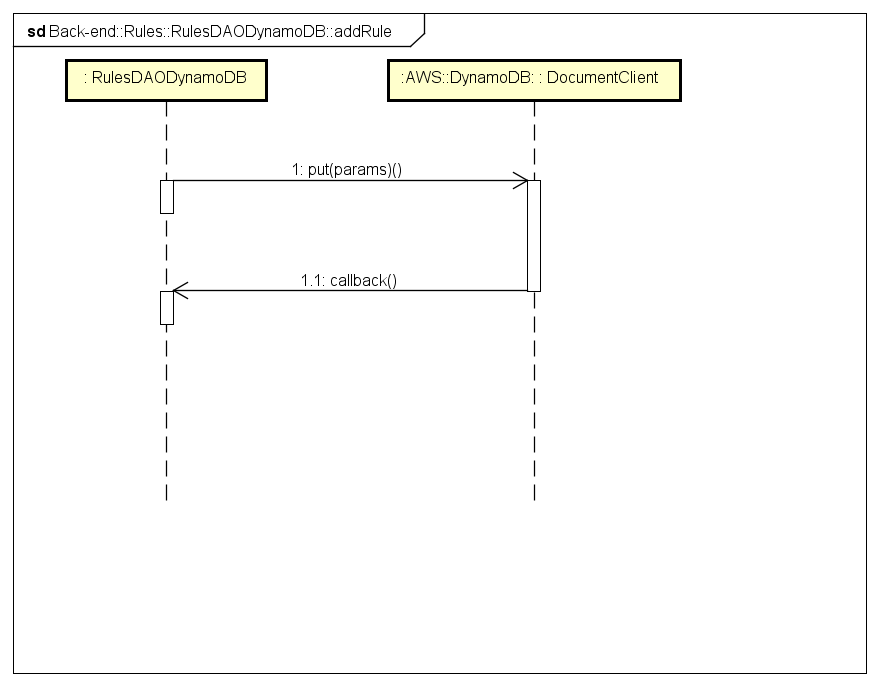
\includegraphics[width=\textwidth,height=\textheight,keepaspectratio]{images/diagrams/back-end/Ufficial_Backend/Back-endRulesRulesDAODynamoDBaddRule.png} 	\caption{Back-end::Rules::RulesDAODynamoDB::addRule}
\end{figure}
\newpage

\subsection{Back-end::Rules::RulesDAODynamoDB::getRule}
Il diagramma qui riportato rappresenta l'ottenimento di una \file{Rule} dal database attraverso il metodo \file{get} del \file{DocumentClient} di \file{DynamoDB}, utilizzando la risposta come parametro per chiamare la funzione di callback.
 \begin{figure}[h] \centering 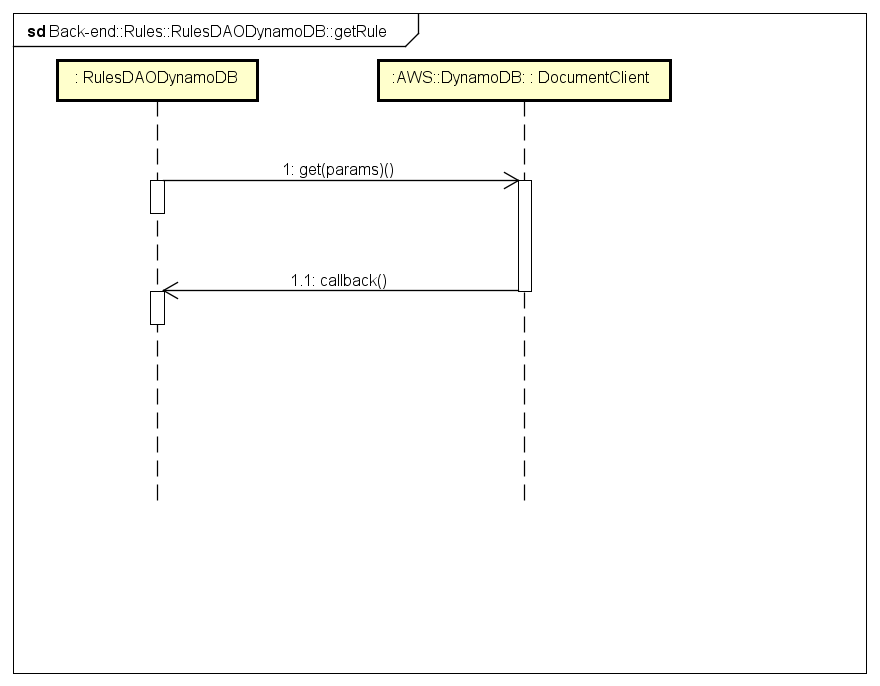
\includegraphics[width=\textwidth,height=\textheight,keepaspectratio]{images/diagrams/back-end/Ufficial_Backend/Back-endRulesRulesDAODynamoDBgetRule.png} 	\caption{Back-end::Rules::RulesDAODynamoDB::getRule}
\end{figure}
\newpage

\subsection{Back-end::Rules::RulesDAODynamoDB::getRuleList}
Il diagramma qui riportato rappresenta l'ottenimento della lista di \file{Rule} dal database attraverso il metodo \file{scan} del \file{DocumentClient} di \file{DynamoDB}, utilizzando la risposta come parametro per chiamare la funzione di callback. Poichè il metodo \file{scan} del \file{DocumentClient} permette al più il ritorno di una lista delle dimensioni di 1MB, se il campo LastEvaluetedKey è settato allora non tutte le \file{Rule} sono state ritornate, e quindi è necessario rieseguire il metodo scan fornendo come parametro d'ingresso la chiave da cui ripartire per l'estrazione dei dati. Se invece tale campo non è settato allora è stata ritornata l'intera lista.
 \begin{figure}[h] \centering 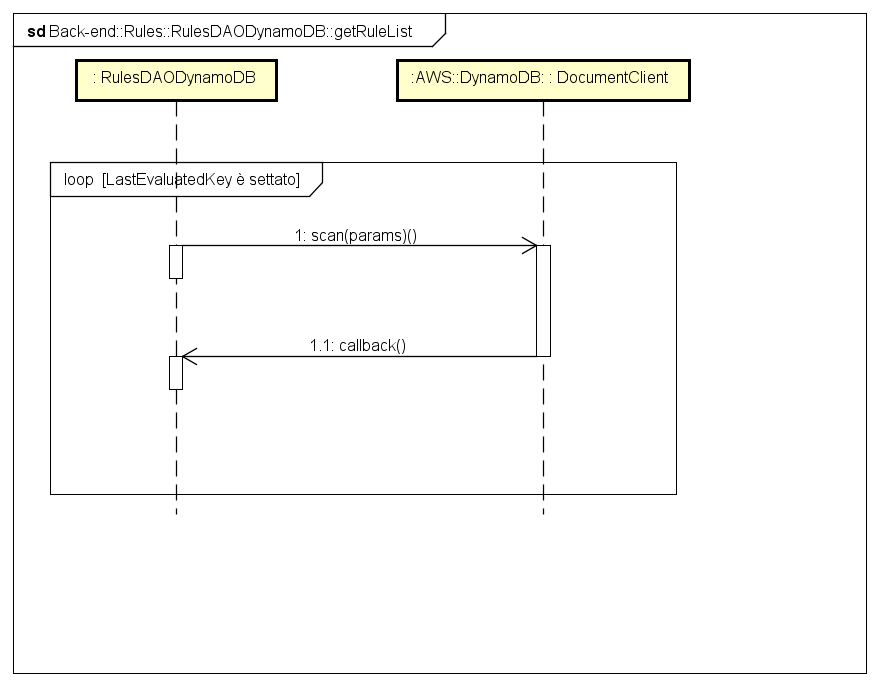
\includegraphics[width=\textwidth,height=\textheight,keepaspectratio]{images/diagrams/back-end/Ufficial_Backend/Back-endRulesRulesDAODynamoDBgetRuleList.png} 	\caption{Back-end::Rules::RulesDAODynamoDB::getRuleList}
\end{figure}
\newpage

\subsection{Back-end::Rules::RulesDAODynamoDB::removeRule}
Il diagramma qui riportato rappresenta la rimozione di una \file{Rule} dal database attraverso il metodo \file{delete} del \file{DocumentClient} di \file{DynamoDB}, utilizzando la risposta come parametro per chiamare la funzione di callback.
 \begin{figure}[h] \centering 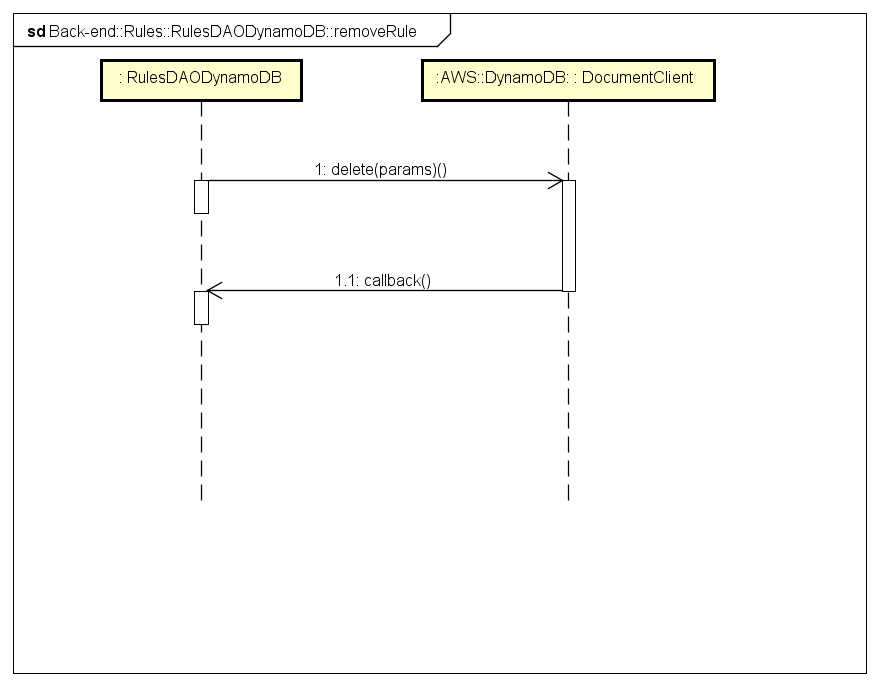
\includegraphics[width=\textwidth,height=\textheight,keepaspectratio]{images/diagrams/back-end/Ufficial_Backend/Back-endRulesRulesDAODynamoDBremoveRule.png} 	\caption{Back-end::Rules::RulesDAODynamoDB::removeRule}
\end{figure}
\newpage

\subsection{Back-end::Rules::RulesDAODynamoDB::updateRule}
Il diagramma qui riportato rappresenta la modifica di una \file{Rule} del database attraverso il metodo \file{update} del \file{DocumentClient} di \file{DynamoDB}, utilizzando la risposta come parametro per chiamare la funzione di callback.
 \begin{figure}[h] \centering 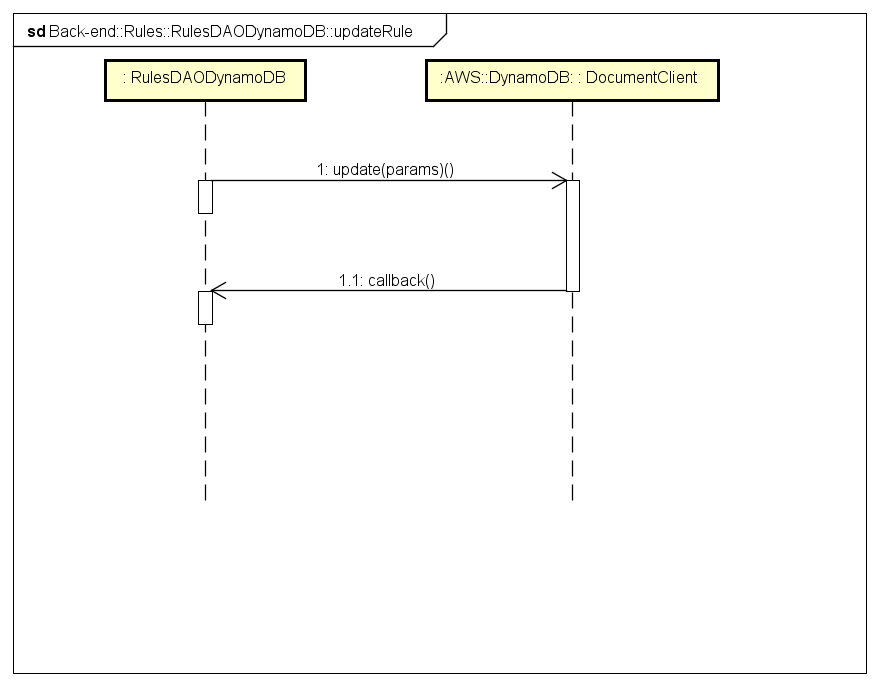
\includegraphics[width=\textwidth,height=\textheight,keepaspectratio]{images/diagrams/back-end/Ufficial_Backend/Back-endRulesRulesDAODynamoDBupdateRule.png} 	\caption{Back-end::Rules::RulesDAODynamoDB::updateRule}
\end{figure}
\newpage

\subsection{Back-end::STT::STTWatsonAdapter::speechToText}
Il diagramma qui riportato rappresenta il riconoscimento di un file audio per mezzo del metodo \file{recognize} fornito dallo \file{SpeechToTextV1} di \file{WatsonDeveloperCloud}.
\begin{figure}[h] \centering 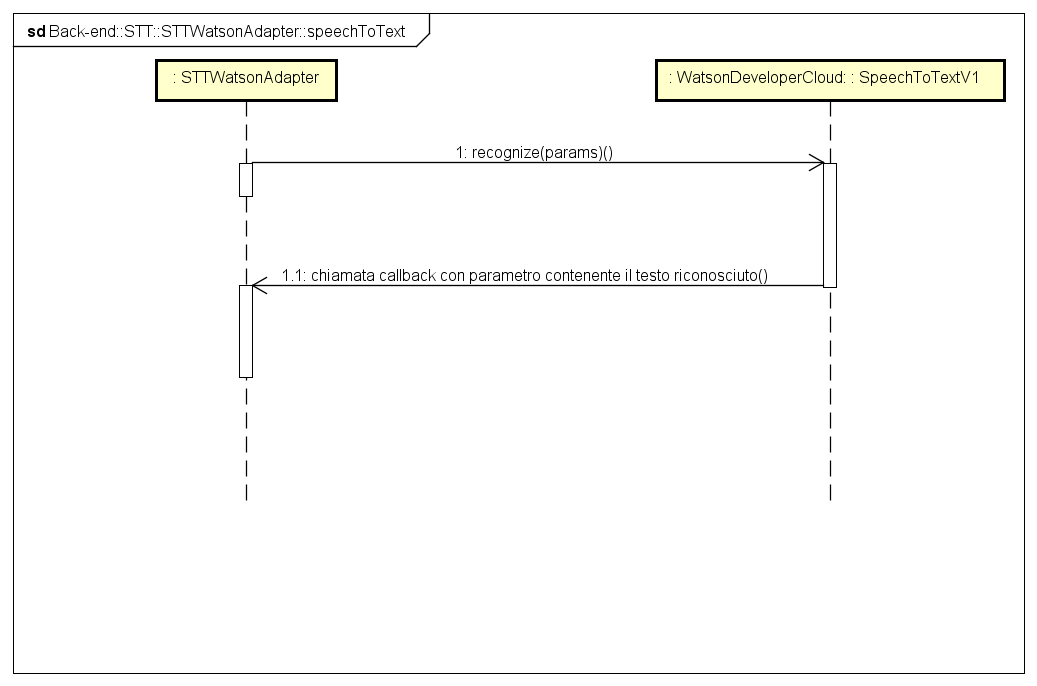
\includegraphics[width=\textwidth,height=\textheight,keepaspectratio]{images/diagrams/back-end/Ufficial_Backend/Back-endSTTSTTWatsonAdapterspeechToText.png} 	\caption{Back-end::STT::STTWatsonAdapter::speechToText}
\end{figure}
